





\begin{abstract}
We perceive speech as a series of relatively invariant phonemes despite extreme variability in the acoustic signal. To be perceived as nearly-identical phonemes, speech sounds that vary continuously over a range of acoustic parameters must be perceptually discretized by the auditory system. Such many-to-one mappings of undifferentiated sensory information to a finite number of discrete categories are ubiquitous in perception. Although many mechanistic models of phonetic perception have been proposed, they remain largely unconstrained by neurobiological data. Current human neurophysiological methods lack the necessary spatiotemporal resolution to provide it: speech is too fast and the neural circuitry involved is too small. Here we demonstrate that mice are capable of learning generalizable phonetic categories, and can thus serve as a model for phonetic perception. Mice learned to discriminate consonants, and generalized consonant identity across novel vowel contexts and speakers, consistent with true category learning. A mouse model, given the powerful genetic and electrophysiological tools for probing neural circuits available for them, has the potential to powerfully augment our mechanistic understanding of phonetic perception.

\end{abstract}

\maketitle

\thanks{Additional thanks to Aldis Weible, Lucas Ott, and Connor O'Sullivan. This material is based upon work supported by the National Science Foundation Graduate Research Fellowship Program under Grant No. 1309047. Any opinions, findings, and conclusions or recommendations expressed in this material are those of the author(s) and do not necessarily reflect the views of the National Science Foundation.}

%
%%%%%%%%%%%%%%%%%%%%%%%%%%%%%%%%%%%%%%%%%%%%%%%%%%%%%%%%%%%%%%%%
%%%%%%%%%%%%%%%%%%%%%%%%%%%%%%%%%%%%%%%%%%%%%%%%%%%%%%%%%%%%%%%%
%
% Introduction
%
%%%%%%%%%%%%%%%%%%%%%%%%%%%%%%%%%%%%%%%%%%%%%%%%%%%%%%%%%%%%%%%%
%%%%%%%%%%%%%%%%%%%%%%%%%%%%%%%%%%%%%%%%%%%%%%%%%%%%%%%%%%%%%%%%
\section{Introduction}
\subsection{Lack of acoustic invariance in phonemes}

We perceive speech as a series of relatively invariant phonemes despite extreme variability in the acoustic signal. This lack of order within phonemic categories remains one of the fundamental problems of speech perception \cite{Sussman1998}. Plosive stop consonants (such as /b/ or /g/) are the paradigmatic example of phonemes with near-categorical perception\cite{Holt2010,Kronrod2016a,LIBERMAN1957} without invariant acoustic structure\cite{Elman1988,Kluender1987}. The problem is not just that phonemes are acoustically variable, but rather that there is a fundamental lack of invariance in the relation between phonemes and the acoustic signal\cite{Kluender1987}. Despite our inability to find a source of invariance in the speech signal, the auditory system learns some acoustic-perceptual mapping such that a plosive stop like /b/ is perceived as nearly identical across phonetic contexts. A key source of variability is coarticulation, which causes the sound of a spoken consonant to be strongly affected by neighboring segments, such as vowels. Coarticulation occurs during stop production because the articulators (such as the tongue or lips) have not completely left the positions from the preceding phoneme, and are already moving to anticipate the following phoneme \cite{Liberman1967,Farnetani1990}.  Along with many other sources of acoustic variation like speaker identity, sex, accent, or environmental noise; coarticulation guarantees that a given stop consonant does not have a uniquely invariant acoustic structure across phonetic contexts. In other words, there is no canonical acoustic /b/\cite{Liberman1967,Holt2010}. Phonetic perception therefore cannot be a simple, linear mapping of some continuous feature space to a discrete phoneme space. Instead it requires a mapping that flexibly uses evidence from multiple, imperfect cues depending on context\cite{Holt2010, Diehl2004}. This invariant perception of phonemes, despite extreme variability in the physical speech signal, is referred to as the non-invariance problem \cite{Perkell1986}.

\subsection{Generality of phonetic perception}

The lack of a simple mapping between acoustic attributes and phoneme identity has had a deep influence on phonetics, in part motivating the hypothesis that speech is mechanistically unique to humans\cite{Lieberman1984}, and the development of non-acoustic theories of speech perception (most notably motor theories\cite{Diehl2004,Liberman1967,Liberman1985}). However, it has been clear for more than 30 years that at least some auditory components of speech perception are not unique to humans, suggesting that human speech perception exploits evolutionarily-preserved functions of the auditory system\cite{Kluender1987,Carbonell2014,Ghazanfar1999,Bornkessel-Schlesewsky2015}. For example, nonhuman animals like quail\cite{Kluender1987, Kluender1994}, chinchillas\cite{Kuhl1978}, rats\cite{Engineer2015}, macaques\cite{Kuhl1983}, and songbirds\cite{Dooling1995} are capable of learning phonetic categories that share some perceptual qualities with humans\cite{Lotto1997,Kluender2000}. This is consistent with the idea that categorizing phonemes is just one instance of a more general problem faced by all auditory systems, which typically extract useable information from complex acoustic environments by reducing them to a small number of 'auditory objects' (for review, see\cite{Bizley2013}).%
%
\subsection{Neurolinguistic theories of phonetic perception}

Many neurolinguistic theories of phonetic perception have been proposed\cite{Rauschecker2009a,Strauss2007,Kluender2013a,Liberman1985,Gaskell1997}, but neurophysiological evidence to support them is limited. One broad class of models follows the paradigm of hierarchical processing first described by Hubel and Weisel in the visual system\cite{Rauschecker2009a,Hubel1962,Strauss2007}. In these models, successive processing stages in the auditory system extract acoustic features with progressively increasing complexity by combining the simpler representations present in preceding stages. Such hierarchical processing is relatively well-supported by experimental data. For example, the responses of neurons in primary auditory cortex (A1) to speech sounds are more diverse than those in inferior colliculus\cite{Ranasinghe2013} (but see \cite{Bartlett2013}). While phoneme identity can be classified post-hoc from population-level activity in A1\cite{Centanni2013,Engineer2008,Steinschneider2003}, neurons in secondary auditory cortical regions explicitly encode higher-order properties of speech sounds \cite{Mesgarani2014,Belin2000a,Chang2010,Pasley2012,Bidelman2013}.

Another class of models proposes that phonemes have no positive acoustic "prototype", and that we instead learn only the acoustic features useful for telling them apart\cite{Kluender2013a}. Theoretically, these discriminative models provide better generalization and robustness to high variance\cite{Ng2002a}. Theories based on discrimination rather than prototype-matching have a long history in linguistics\cite{Saussure1916}, but have rarely been implemented as neurolinguistic models. A possible neural implementation of discriminative perception is that informative contrast cues could evoke inhibition to suppress competing phonetic percepts, similar to predictive coding \cite{Rutishauser2015,Kluender2013a,Dresher2008}. Neurophysiological evidence supports the existence of discriminative predictive coding, but its specific implementation is unclear\cite{Blank2016,Gagnepain2012}.

These two very different classes of models illustrate a major barrier faced by phonetic research: both classes can successfully predict human categorization performance, making it difficult to empirically validate or refute either of them using psychophysical experiments alone. Mechanistic differences have deep theoretical consequences --- for example, the characterizations made by the above two classes of models regarding what phonemes \textit{are} precisely oppose one another: are they positive acoustic prototypes, or sets of negative acoustic contrasts? Perceptually, do listeners identify phonemes, or discriminate between them? Neurobiological evidence regarding how the brain actually solves these categorization problems could help overcome this barrier.

\subsection{The utility of a mouse model for speech research}

Neurolinguistic research in humans faces several limitations that could be overcome using animal models.

First, most current human neurophysiological methods lack the spatiotemporal resolution to probe the fine spatial scale of neuronal circuitry and the millisecond timescale of speech sounds. A causal, mechanistic understanding of computation in neural circuits is also greatly aided by the ability to manipulate individual neurons or circuit components, which is difficult in humans. Optogenetic methods available in mice provide the ability to activate, inactivate, or record activity from specific types of neurons at the millisecond timescales of speech sounds.

Second, it is difficult to isolate the purely auditory component of speech perception in humans. Humans can use contextual information from syntax, semantics or task structure to infer phoneme identity\cite{Fox2016,Schouten2003}. It is also difficult to rule out the contribution of multimodal information\cite{Rosenblum2008}, or of motor simulation predicted by motor theories. Certainly, these and other non-auditory strategies are used during normal human speech perception. Nevertheless, speech perception is possible without these cues, so any neurocomputational theory of phonetic perception must be able to explain the purely auditory case. Animal models allow straightforward isolation of purely auditory phonetic categorization without interference from motor, semantic, syntactic, or other non-auditory cues.

Third, it is difficult to control for prior language experience in humans. Experience-dependent effects on phonetic perception are present from infancy\cite{Kuhl1992}. It can therefore be challenging to separate experience-driven effects from innate neurocomputational constraints imposed by the auditory system. Completely language-naive subjects (such as animals) allow the precise control of language exposure, permitting phonetics and phonology to be disentangled in neurolinguistics.

Animal models of phonetic perception are a useful way to avoid these confounds, and provide an important alternative to human studies for empirically grounding the development of neurolinguistic theories. The mouse is particularly well-suited to serve as such a model. A growing toolbox of powerful electrophysiological and optogenetic methods in mice has allowed unprecedented precision in characterizing neural circuits and the computations they perform.

\subsection{The utility of phonetics for auditory neuroscience}

Conversely, auditory neuroscience stands to benefit from the framework provided by phonetics for studying how sound is transformed to meaning. Understanding how complex sounds are encoded and processed by the auditory system, ultimately leading to perception and behavior, remains a challenge for auditory neuroscience. For example, it has been difficult to extrapolate from simple frequency/amplitude receptive fields to understand the hierarchical organization of complex feature selectivity across brain areas. A great strength of neuroethological model systems such as the songbird is that both the stimulus (e.g., the bird's own song) and the behavior (song perception and production) are well understood. This has led to significant advances in understanding the hierarchical organization and function of the song system \cite{Brenowitz1997,Theunissen2014}. The long history of of speech research in humans has produced a deep understanding of the relationships between acoustic features and phonetic perception \cite{Peterson1952}. These insights have enabled specific predictions about what kinds of neuronal selectivity for features (and combinations of features) might underlie phonetic perception \cite{Sussman1998}. Although recognizing human speech sounds is not a natural ethological behavior for mice, phonetics nevertheless provides a valuable framework for studying how the brain encodes and transforms complex sounds into perception and behavior.

Here we trained mice to discriminate between pitch-shifted recordings of naturally produced consonant-vowel (CV) pairs beginning with either /g/ or /b/. Mice demonstrated the ability to generalize consonant identity across novel vowel contexts and speakers, consistent with true category learning. To our knowledge this is the first demonstration that any animal can generalize consonant identity across both novel vowel contexts and novel speakers. These results indicate that mice can solve the non-invariance problem, and suggest that mice are a suitable model for studying phonetic perception.

%%%%%%%%%%%%%%%%%%%%%%%%%%%%%%%%%%%%%%%%%%%%%%%%%%%%%%%%%%%%%%%%
%%%%%%%%%%%%%%%%%%%%%%%%%%%%%%%%%%%%%%%%%%%%%%%%%%%%%%%%%%%%%%%%
%
% Results
%
%%%%%%%%%%%%%%%%%%%%%%%%%%%%%%%%%%%%%%%%%%%%%%%%%%%%%%%%%%%%%%%%
%%%%%%%%%%%%%%%%%%%%%%%%%%%%%%%%%%%%%%%%%%%%%%%%%%%%%%%%%%%%%%%%

\section{\Large Results}

\subsection{Generalization performance}

\begin{figure}
\includegraphics[width=\linewidth]{speech/figures/Figure1.pdf}
\caption{\textbf{Stimuli and Task Design.} \textbf{a)} Spectrograms of stimuli. Left: Example of an original recording of an isolated consonant-vowel token (/gI/). Center: the same token pitch-shifted upwards by 10x (3.3 octaves) into the mouse hearing range. Right: Recording of the pitch-shifted token presented in the behavior box. Stimuli retained their overall acoustic structure below 34kHz (the upper limit of the speaker frequency response). \textbf{b)} Power spectra (dB, Welch's method) of tokens in \textbf{a}. Black: Original (left frequency axis), red: Pitch-shifted (right frequency axis), blue: Box Recording (right frequency axis). \textbf{c)} Mice initiated a trial by licking in a center port and responded by licking on one of two side ports. Correct responses were rewarded with water and incorrect responses were punished with a mildly-aversive white noise burst. \textbf{d)} The difficulty of the task was gradually expanded by adding more tokens (squares), vowels (labels), and speakers (rows) before the mice were tested on novel tokens in a generalization task. \textbf{e)} Mice (colored lines) varied widely in the duration of training required to reach the generalization phase. Mice were returned to previous levels if they remained at chance performance after reaching a new stage.
}
\label{spectro}
\end{figure}
%%%%%%%%%%%%%%%%%%%%%%%%%%%%%%%%%%%%%%%%%%%%%%%%%%%%%%%%%%%%%%%%
%
% General Performance Figure
%
%%%%%%%%%%%%%%%%%%%%%%%%%%%%%%%%%%%%%%%%%%%%%%%%%%%%%%%%%%%%%%%%
%

\begin{figure}
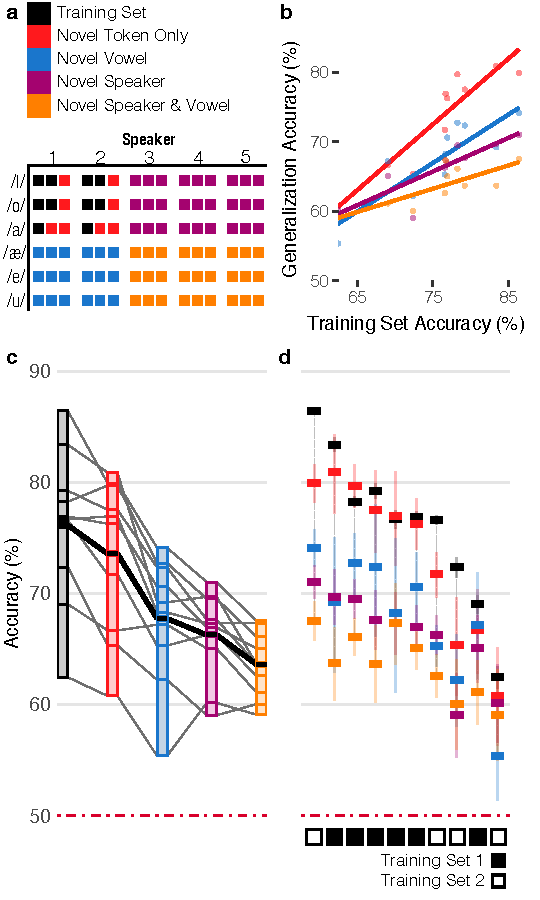
\includegraphics[width=\linewidth]{speech/figures/Figure2.pdf}
\caption{\textbf{Generalization accuracy by novelty class.} Mice generalized stop consonant discrimination to novel CV recordings. \textbf{a)} Four types of novelty are possible with our stimuli: novel tokens from the speakers and vowels used in the training set (red), novel vowels (blue), novel speakers (purple), and novel speakers with novel vowels (orange). Tokens in the training set are indicated in black. Colors same throughout. \textbf{b)} Mice that performed better on the training set were better at generalization. Each point shows the performance for a single mouse on a given novelty class, plotted against that mouse's performance on training tokens presented on during the generalization phase (both averaged across the entire generalization phase). Lines show linear regression for each novelty class. \textbf{c)} Mean accuracy for each novelty class (gray lines indicate individual mice). \textbf{d)} Mean accuracy for individual mice (colored bars indicate each novelty class). Error bars in \textbf{d} are 95\% binomial confidence intervals. Mice were assigned one of two sets of training tokens, black and white boxes in \textbf{d}.}
\label{gen}
\end{figure}

We began training 23 mice to discriminate between consonant-vowel (CV) pairs beginning with either /b/ or /g/ in a two-alternative forced choice task. CV tokens were pitched-shifted up into the mouse hearing range (Fig. \ref{spectro}a-b). Each mouse began training with a pair of tokens (individual recordings) in a single vowel context (ie. /bI/ and /gI/) from a single speaker, and then advanced through stages that progressively introduced new tokens, vowels, and speakers (Fig. \ref{spectro}c-d, see Methods). Training was discontinued in 13 (56.5\%) of these mice because their performance on the first stage was not significantly better than chance after two months. The remaining 10 (43.5\%) mice progressed through all the training stages to reach a final generalization task, on average in 14.9 ($\sigma\pm 7.8$) weeks (Fig. \ref{spectro}e). This success rate and training duration suggest that the task is difficult but achievable. 

We note that this training time is similar to that reported previously for rats (14$\pm 0.3$ weeks\cite{Engineer2015}). Previous studies have not generally reported success rates. Human infants also vary in the rate and accuracy of their acquisition of phonetic categories\cite{Werker1988}, so we did not expect perfect accuracy from every mouse. The cause of such differences in ability is itself an opportunity for future study.

Generalization is an essential feature of categorical perception. By testing whether mice can generalize their phonetic categorization to novel stimuli, we can distinguish whether mice actually learn phonetic categories or instead just memorize the reward contingency for each training token. Four types of novelty are possible with our stimuli: new tokens from the speakers and vowel contexts used in the training set, new vowels, new speakers, and new vowels from new speakers (colored groups in Fig. \ref{gen}a). In the final generalization stage, we randomly interleaved tokens from each of these novelty classes on 20\% of trials, with the remaining 80\% consisting of tokens from the training set. We interleaved novel tokens with training tokens for two reasons: (1) to avoid a sudden increase in task difficulty, which can degrade performance, and (2) to minimize the possibility that mice could learn each new token by widely separating them in time (on average, generalization tokens were repeated only once every five days).

We looked for 4 hallmarks of generalization: (1) Mice should be able to accurately categorize novel tokens, (2) performance should reflect the quality of the acoustic-phonetic criteria learned in training, (3) performance on novel tokens should be correspondingly worse for tokens that differ more from those in the training set, and (4) accurate categorization of novel tokens should not require additional reinforcement.

All 10 mice were able to categorize tokens of all generalization types with an accuracy significantly greater than chance. We estimated the impact of each generalization class on performance as a fixed factor nested within each mouse as a random factor in a mixed-effects logistic regression (see Methods). The predicted accuracy for each generalization class is shown in Table \ref{lmmtab}, each providing an estimate of the difficulty of that class after accounting for the random effects of individual mice.

Performance on all generalization types was strongly and positively correlated with performance on the training set (Fig. \ref{gen}b, adj. $R^2$=0.74, F(4, 5) = 7.4, $p <$ 0.05). If mice were "overfitting," that is, memorizing the training tokens rather than learning categories, then we would expect the opposite (i.e., above some threshold, mice that performed better on the training set would perform correspondingly worse on the generalization set). It appears instead that better prototypes or decision boundaries learned in the training stages allowed better generalization to novel tokens.

Mice were better at some types of generalization than others (Fig. \ref{gen}c). The estimates of their relative difficulty (Fig. \ref{gen}c) provide a ranking of the perceptual novelty of the stimulus classes based on their similarity to the training tokens. From easiest to hardest, these were: novel token, novel vowel, novel speaker (which was not significantly more difficult than novel vowel), novel speaker \& vowel. The effects of generalizing to novel vowels and novel speakers were not significantly different from each other, but pairwise comparisons between each of the other types of generalization were (Tukey's method, all $p < 0.001$, also see confidence intervals in Table \ref{lmmtab}).

Although the effect of each generalization type on performance was significantly different between mice (Likelihood Ratio Test, $\chi^2$(14) = 407.22, $p \ll 0.001$), they were highly correlated (see Table \ref{lmmtab}). The relative consistency of novelty type difficulty across mice (ie. the correlation of fixed effects, Fig. \ref{gen}c) is striking, but our results cannot distinguish whether it is due to the mice or the stimuli: it is unclear whether the acoustic/phonetic criteria learned by all mice are similarly general, or whether the "cost" of each type of generalization is similar across an array of possible acoustic/phonetic criteria.


\begin{figure}
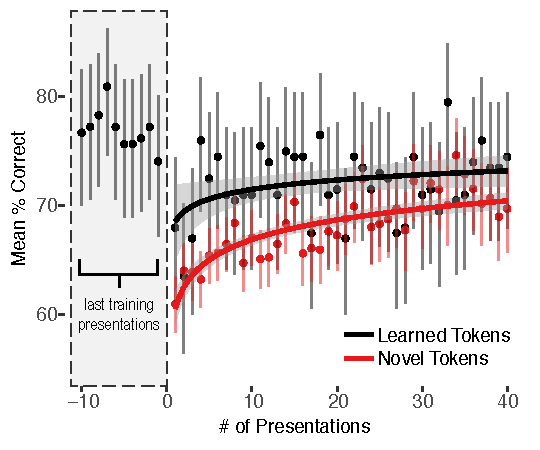
\includegraphics[width=\linewidth]{speech/figures/Figure3.pdf}
\caption{\textbf{Learning curve for novel tokens.} Performance for both novel and training set tokens dropped transiently and recovered similarly after the transition to the generalization stage. Presentation 0 corresponds to the transition to the generalization stage. The final ten trials before the transition are shown in the gray dashed box. Mean accuracy and 95\% binomial confidence intervals are collapsed across mice for novel (red, all novelty classes combined) or learned (black) tokens, by number of presentations in the generalization task. Logistic regression of binomial correct/incorrect responses fit to log-transformed presentation number (lines, shading is smoothed standard error).}
\label{lc}
\end{figure}

True generalization requires that one set of discrimination criteria can be successfully applied to novel cases without reinforcement. It is possible that the mice were instead able to rapidly learn the reward contingency of novel tokens during the generalization stage. If mice were learning rapidly rather than generalizing, this would predict that novel token performance (1) would be indistinguishable from chance on the first presentation, and (2) would increase relative to performance on already-learned tokens with repeated presentations.

Performance on the first presentation of novel tokens was significantly greater than chance (Fig. 3, all mice, all tokens from all novelty classes: one-sided binomial test, n=1410, $P_{correct}$ = 0.61, lower 95\% CI = 0.588, p $\ll$ 0.001; all mice, worst novelty class:  n=458, $P_{correct}$ = 0.581, lower 95\% CI = 0.541, p $<$ 0.001). This demonstrates that mice were able to generalize immediately without additional reinforcement. Although performance on novel tokens did increase with repetition, so did performance on training tokens (Fig. \ref{lc}). We noted that performance on all tokens (both novel and previously learned tokens) transiently dropped after each transition between task stages, suggesting a non-specific effect of an increase in task difficulty. To distinguish an increase in performance due to learning from an increase due to acclimating to a change in the task, we compared performance on generalization and training tokens over the first 40 presentations of each token. If the mice were learning the generalization tokens, the increase in performance with repeated presentations should be significantly greater than that of the already trained tokens.

Performance was well fit by a logistic regression of correct/incorrect responses from each mouse against the novelty of a token (trained vs. novel tokens), and the number of times it had been presented (Fig. \ref{lc}). The effect of the number of presentations on accuracy was not significantly different for novel tokens compared to trained tokens (interaction between novelty and the number of presentations: Wald test, z = 1.239, 95\% CI = [-0.022, 0.1], p=0.215). This was also true when the model was fit with with the generalization types themselves rather than trained vs. novel tokens (most significant interaction, generalization to novel speakers x number of presentations: Wald test, z = 1.425, 95\% CI = [-0.018, 0.117], p=0.154) and with different numbers of repetitions (10: z = -0.219, 95\% CI = [-0.161, 0.13], p=0.827; 20: z = -0.521, 95\% CI = [-0.116, 0.068], p=0.602). This indicates that the asymptotic increase in performance on novel tokens was a general effect of adapting to a change in the task rather than a learning period for the novel stimuli.

In summary, the behavior of the mice is consistent with an ability to generalize some learned acoustic criteria to novel stimuli. It is unlikely that the mice rapidly learned the novel tokens because (1) performance on the first presentation of novel tokens was significantly above chance, (2) performance on subsequent presentations of novel tokens did not improve compared to trained tokens, and (3) learning each token would have to take place over unrealistically long timescales: there were an average of 2355 trials (5 days) between the first and second presentation of each novel token.

\subsection{Training Set Differences}

%%%%%%%%%%%%%%%%%%%%%%%%%%%%%%%%%%%%%%%%%%%%%%%%%%%%%%%%%%%%%%%%
%
% Heatmap Figure
%
%%%%%%%%%%%%%%%%%%%%%%%%%%%%%%%%%%%%%%%%%%%%%%%%%%%%%%%%%%%%%%%%
%
%
One strength of studying phonetic perception in animal models is the ability to precisely control exposure to speech sounds. To test whether and how the training history impacted the pattern of generalization, we divided mice into two cohorts trained with different sets of speech tokens. In the first cohort (n = 6 mice), mice were trained with tokens from speakers 1 and 2 (speaker number in Fig. \ref{heat}a), whereas the second cohort (n = 4 mice) were trained on speakers 4 and 5.


\begin{figure}[ht]
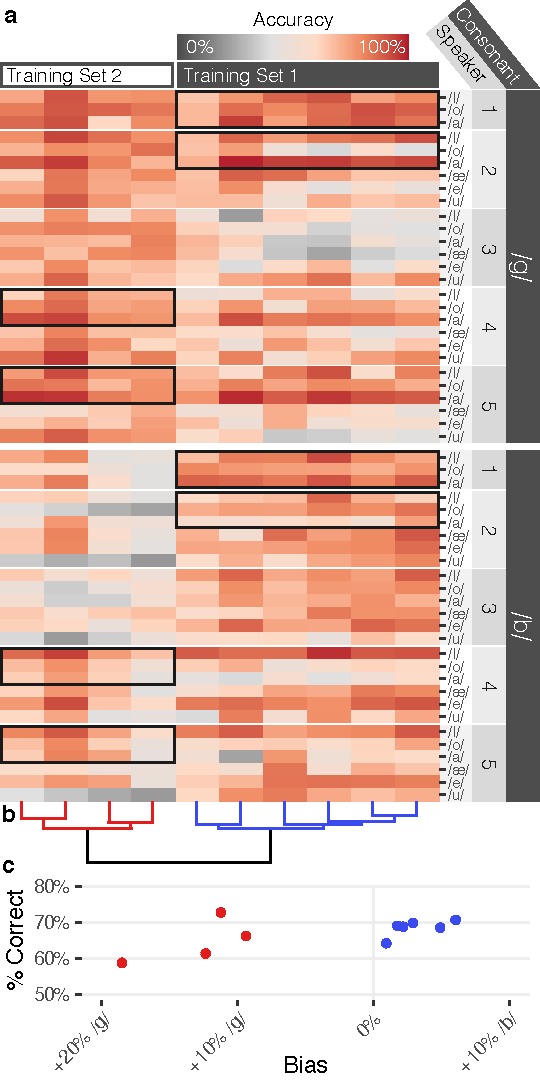
\includegraphics[width=\linewidth]{speech/figures/Figure4.pdf}
\caption{\textbf{Patterns of individual and group variation.} \textbf{a)}Mean accuracy (color, scale at top) for each mouse (columns) on tokens grouped by consonant, speaker, and vowel (rows). The different training sets (cells outlined with black boxes) led to different patterns of accuracy on the generalization set. \textbf{b)} Ward clustering dendrogram, colored by cluster. \textbf{c)} Training set cohorts differed in bias but not mean accuracy.
}
\label{heat}
\end{figure}

The two training cohorts had significantly different patterns of which tokens were accurately categorized (Fig. \ref{heat}a, Likelihood-Ratio test, regression of mean accuracy on tokens with and without token x cohort interaction: $\chi^2_{161}$, $p \ll 0.001$). Put another way, accuracy patterns were markedly similar within training cohorts: cohort differences accounted for fully 40.6\% of all accuracy variance (sum of squared-error) between tokens.

Mice from the second training cohort were far more likely to report novel tokens as a /g/ than the first cohort (Fig. \ref{heat}b), an effect that was not significantly related to their overall accuracy (b=0.351, $t(8)=2.169$, p=0.062 ). Since the only difference between these mice were the tokens they were exposed to during training (they were trained contemporaneously in the same boxes),  we interpret this response bias as the influence of the training tokens on whatever acoustic cues the mice had learned in order to perform the generalization task. This suggests that the acoustic properties of training set 2 caused the /g/ "prototype" to be overbroad.

We searched for additional sub-cohort structure with hierarchical clustering (Ward's Method, dendrogram in fig \ref{heat}b). Within each training cohort there appeared to be two additional clusters of accuracy patterns. Though our sample size was too small to meaningfully interpret these clusters, they raise the possibility that even when trained using the same set of sounds mice might learn multiple sets of rules to distinguish between consonant classes.


%%%%%%%%%%%%%%%%%%%%%%%%%%%%%%%%%%%%%%%%%%%%%%%%%%%%%%%%%%%%%%%%
%
% Acoustic-Behavioral Correlates
%
%%%%%%%%%%%%%%%%%%%%%%%%%%%%%%%%%%%%%%%%%%%%%%%%%%%%%%%%%%%%%%%%
%
\subsection{Acoustic-behavioral correlates}


\begin{figure}[!t]
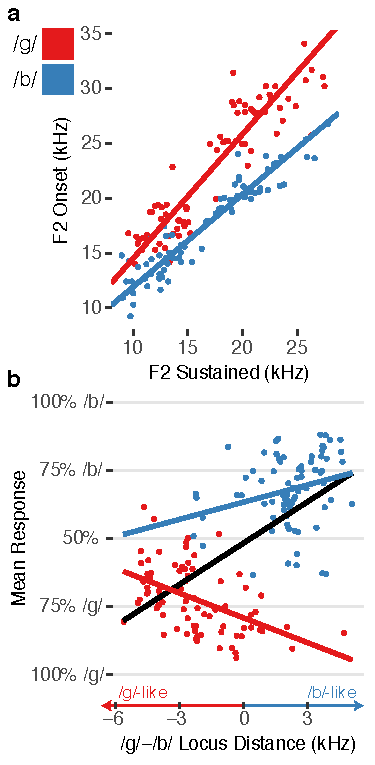
\includegraphics[width=2.5in]{speech/figures/Figure5.pdf}
\caption{\textbf{Acoustic-Behavior Correlates} F2 Onset-Vowel transitions do not explain observed response patterns. \textbf{a)} Locus equations relating F2 at burst onset and vowel steady state (sustained) for each token (points), split by consonant (colors, same as \textbf{b)}). \textbf{b)} As the difference of a token's distance from the ideal /g/ and /b/ locus equation lines increased (x axis, greater distance from /g/, smaller distance from /b/), /b/ tokens obeyed the predicted categorization while /g/ tokens did not (slopes of colored lines). }
\label{acoustic}
\end{figure}

Humans can flexibly use several acoustic features such as burst spectra and formant transitions to discriminate plosive consonants, and we wondered to what extent mice were sensitive to these same features.

One dominant acoustic cue for place of articulation in stop consonants is the transition of the second formant following the plosive burst\cite{Wright2004,Sussman1998,Lindblom2012}. Formant transitions are complex and dependent on vowel context, but tokens for a given place of articulation cluster around a line -- or "locus equation" -- relating F2 frequency at release to its mid-vowel steady-state\cite{Sussman1998,Lindblom2012} (Fig. \ref{acoustic}a).  If mice were sensitive to this cue, the distance from both locus equation lines should influence response. For example, a /g/ token between the locus equation lines should have a greater rate of misclassification than a token at an equal distance above the red /g/ line. Therefore we tested how classification depended on the difference of distances from each line (/g/ distance - /b/ distance, which we refer to as "locus difference").

Mean responses to tokens (ranging from 100\% /g/ - 100\% /b/) were correlated with locus differences (black line, Fig. \ref{acoustic}b). However, it is important to note that this correlation does not necessarily demonstrate that mice relied on this acoustic cue. Because multiple acoustic features are correlated with consonant identity, performance that is correlated with one such cue would also be correlated with all the others.
The mice learned some acoustic property of the consonant classes, and since the acoustic features are all highly correlated with one another, they are all likely to correlate with mean responses.
To distinguish whether mice specifically relied on F2 locus distance, we therefore measured the marginal effect of this acoustic cue within a consonant class. This is shown by the slopes of the red and blue lines in Fig. \ref{acoustic}b. For example, is a /g/ token that is further away from the blue /b/ line more likely to be identified as a /g/ than one very near the /b/ line? Mean responses to /g/ tokens were negatively correlated with locus distance (Mean response /g/ to /b/ between 0 and 1, b=-0.028kHz, 95\% CI = [-0.035, -0.022], $p \ll 0.001$). In other words, tokens that should have been more frequently confused with /b/ were actually more likely to be classified as /g/. Note the red points at locus distance of zero in Fig. \ref{acoustic}b: these tokens have an equal distance from both the /b/ and /g/ locus equation prototypes but are some of the most accurately categorized /g/ tokens. /b/ tokens obeyed the predicted direction of locus distance (b=0.049, 95\% CI = [0.039, 0.06], $p \ll 0.001$), but the effect was very small: moving one standard deviation ($\sigma_{/b/}$=1.618kHz) towards the /g/ line only changed responses by 7.9\%. These results suggest that mice did not rely on F2 transitions to categorize these consonants.

We repeated this analysis separately for each training cohort to test whether the two cohorts could have developed different acoustic templates that better explained their response patterns. We derived cohort-specific locus-equation lines and distances using only the tokens from each of their respective training sets. These models were qualitatively similar to the model that included all tokens and mice and did not improve the model fit (Cohort 1: /g/: $b=-0.051, 95\% CI = [-0.064, -0.038]$, /b/: $b=0.041, 95\% CI = [0.022, 0.059]$; Cohort 2: /g/: $b=-0.022, 95\% CI = [-0.031, -0.014]$, /b/: $b=0.055, 95\% CI = [0.042, 0.069]$).

We conclude that while our stimulus set had the expected F2 formant transition structure, this was unable to explain the behavioral responses we observed both globally and within training cohorts. There are, of course, many more possible acoustic parameterizations to test, but the failure of F2 transitions to explain our behavioral data is notable because of its perceptual dominance in humans and its common use in parametrically synthesized speech sounds. This demonstrates one advantage of using natural speech sounds: mice trained on synthesized speech that varied parametrically only on F2 transitions would likely show sensitivity to this cue, but this does not mean that mice show the same feature sensitivity when trained with natural speech. Preserving the complexity of natural speech stimuli is important for developing a general understanding of auditory category learning.

%%%%%%%%%%%%%%%%%%%%%%%%%%%%%%%%%%%%%%%%%%%%%%%%%%%%%%%%%%%%%%%%
%%%%%%%%%%%%%%%%%%%%%%%%%%%%%%%%%%%%%%%%%%%%%%%%%%%%%%%%%%%%%%%%
%
% Discussion
%
%%%%%%%%%%%%%%%%%%%%%%%%%%%%%%%%%%%%%%%%%%%%%%%%%%%%%%%%%%%%%%%%
%%%%%%%%%%%%%%%%%%%%%%%%%%%%%%%%%%%%%%%%%%%%%%%%%%%%%%%%%%%%%%%%

\section{\Large Discussion}

These results demonstrate that mice are capable of learning and generalizing phonetic categories. Indeed, this is the first time to our knowledge that mice have been trained to discriminate between any classes of natural, non-species-specific sounds. Thus mice join a number of model organisms that have demonstrated categorical learning with speech sounds\cite{Kluender1987,Lotto1997,Kluender2000,Kuhl1978,Engineer2015,Kuhl1983,Dooling1995}, making a new suite of genetic and electrophysiological tools available for phonetic research.

Two subgroups of our mice that were trained using different sets of speech tokens demonstrated distinct patterns of consonant identification, presumably reflecting differences in underlying acoustic prototypes. The ability to precisely control exposure to speech sounds provides an opportunity to probe the neurocomputational constraints that govern the possible solutions to consonant identification.

Here we opted to use naturally recorded speech tokens in order to demonstrate that mice could perform a "hard version" of phonetic categorization that preserves the full complexity of the speech sounds and avoids \textit{a priori} assumptions about the parameterization of phonetic contrasts. Although our speech stimuli had the expected F2 formant transition structure, that did not explain the response patterns of our mice. This suggests that the acoustic rules that mice learned are different from those that would be learned from synthesized speech varying only along specifically chosen parameters.

Future experiments using parametrically synthesized speech sounds are a critical next step, and will support a qualitatively different set of inferences. Being able to carefully manipulate reduced speech sounds is useful to probe the acoustic cue structure of learned phonetic categories, but the reduction in complexity that makes them useful also makes it correspondingly more difficult to probe the learning and recognition mechanisms for a perceptual category that is defined by multiple imperfect, redundant cues. It is possible that the complexity of natural speech may have caused our attrition rate to be higher, and task performance lower, than other sensory-driven tasks. Neither of those concerns, however, detracts from the possibility for the mouse to shed mechanistic insight on phonetic perception. Indeed, error trials may provide useful neurophysiological data about how and why the auditory system fails to learn or perceive phonetic categories.

We hope in future experiments to directly test predictions made by neurolinguistic models regarding phonetic acquisition and discrimination. For example, one notable model proposes that consonant perception relies on combination-sensitive neurons that selectively respond to specific combinations of acoustic features \cite{Sussman1998}. This model predicts that mice trained to discriminate stop consonants would have neurons selective for the feature combinations that drive phoneme discrimination, perhaps in primary or higher auditory cortical areas. Combination-selective neurons have been observed in A1\cite{Sadagopan2009,Wang2005a}, and speech training can alter the response properties of A1 neurons in rats\cite{Engineer2015}, but it is unclear whether speech training induces combination-selectivity that would facilitate phonetic discrimination.

The ability to record from hundreds of neurons in awake behaving animals using tetrode electrophysiology or 2-photon calcium imaging presents exciting opportunities to test predictions like these. Should some candidate population of cells be found with phonetic selectivity, the ability to optogenetically activate or inactivate specific classes of neurons (such as excitatory or inhibitory cell types, or specific projections from one region to another) could shed light on the circuit computations and transformations that confer that selectivity.

%
%%%%%%%%%%%%%%%%%%%%%%%%%%%%%%%%%%%%%%%%%%%%%%%%%%%%%%%%%%%%%%%%
%%%%%%%%%%%%%%%%%%%%%%%%%%%%%%%%%%%%%%%%%%%%%%%%%%%%%%%%%%%%%%%%
%
% Methods
%
%%%%%%%%%%%%%%%%%%%%%%%%%%%%%%%%%%%%%%%%%%%%%%%%%%%%%%%%%%%%%%%%
%%%%%%%%%%%%%%%%%%%%%%%%%%%%%%%%%%%%%%%%%%%%%%%%%%%%%%%%%%%%%%%%
%
\section{\Large Methods}

\subsection{Animals}

All procedures were performed in accordance with National Institutes of Health guidelines, as approved by the University of Oregon Institutional Animal Care and Use Comittee.

We began training 23 C57BL/6J mice to discriminate and generalize stop consonants in CV (consonant-vowel) pairs. 13 mice failed to learn the task (see Training, below). 10 mice (43.5\%) progressed through all training stages and reached the generalization task in an average 14.9 ($\sigma = 7.8$) weeks. Mean age at training onset was 8.1 ($\sigma$ = 2) weeks, and at discontinuation of training was 50.6 ($\sigma$ = 11.2) weeks. Sex did not significantly affect the probability of passing or failing training (Fisher's Exact Test: $p = 0.102$), nor did the particular behavioral chamber used for training ($p = 0.685$), nor age at the start of training (Logistic regression: $z = 1.071$, $p=0.284$). Although this task was difficult, our training time (14$\pm 0.3$ weeks as in \cite{Engineer2015}), and accuracy (generalization: 76\%\cite{Kluender1987}, training tokens only: 84.1\% \cite{Engineer2015}) are similar to comparable experiments in other animals.

\subsection{Speech stimuli}

Speech stimuli were recorded in a sound-attenuating booth with a head-mounted microphone attached to a Tascam DR-100mkII handheld recorder sampling at 96kHz/24bit. Each speaker produced a set of 3 recordings (tokens) of each of 12 CV pairs beginning with either /b/ or /g/, and ending with /I/, /o/, /a/, /\ae/, /$\varepsilon$/, /u/. To reduce a slight hiss that was present in the recordings, they were denoised using a Daubechies wavelet with two vanishing moments in MATLAB. The typical human hearing range is 20 Hz - 20 kHz, whereas the mouse hearing range is ~1 kHz - 80 kHz \cite{Radziwon2009}. The $F_0$ of our recorded speech sounds ranged from 100 - 200 Hz, which is well below the lower frequency limit of the mouse hearing range. We therefore pitch shifted all stimuli upwards by 10x (3.3 octaves) in MATLAB\cite{Mathworks}. This shifted all spectral information equally upwards into an analogous part of mouse hearing range while preserving temporal information unaltered.

Tokens from five speakers (one male - speaker 1 throughout, four female - speakers 2-5 throughout) were used. Three vowel contexts (/\ae/, /$\varepsilon$/, and /u/) were not recorded from one speaker. It is unlikely that this had any effect on our results, as our primary claims are based on the ability to generalize at all, rather than generalization to tokens from a particular speaker. Tokens were normalized to a common mean amplitude, but were otherwise unaltered to preserve natural variation between speakers --- indeed, preserving such variation was the reason for using naturally recorded rather than synthesized speech.

Formant frequency values were measured manually using Praat\cite{Boersma2001}. F2 at onset was measured at its center as soon as it was discernible, typically within 20 ms of burst onset, and at vowel steady-state, typically 150-200ms after burst onset.

\subsection{Training}

We trained mice to discriminate between CV pairs beginning with /b/ or /g/ in a two-alternative forced choice task. Training sessions lasted approximately 1 hour, 5 days a week. Each custom-built sound-attenuating training chamber contained two free-field JBL Duet speakers for stimulus presentation with a high-frequency rolloff of 34 kHz, and a smaller 15 x 30 cm plastic box with three "lick ports." Each lick port consisted of a water delivery tube and an IR beam-break sensor mounted above the tube. Beam breaks triggered water delivery by actuating a solenoid valve. Water-restricted mice were trained to initiate each trial with an unrewarded lick at the center port, which started playback of a randomly selected stimulus, and then to indicate their stimulus classification by licking at one of the ports on either side. Tokens beginning with /g/ were always on the left, with /b/ on the right. Two cohorts were trained on two separate sets of tokens. Training set 1 started with speaker 1 (Fig. 4a) and had speaker 2 introduced on the fourth stage, where Training set 2 started training with speaker 5 and had speaker 4 introduced on the fourth stage. Correct classifications received \SI{\sim10}{\micro\liter} water rewards, and incorrect classifications received a 5s time-out that included a mildly aversive 60 dB SPL white noise burst.

Training advanced in stages that progressively increased the number of tokens, vowel contexts, and speakers. Mice first learned a simple pure-tone frequency discrimination task to familiarize them with the task and shape their behavior; the tones were gradually replaced with the two CV tokens of the first training stage. CV discrimination training proceeded in 5 stages outlined in Table 2. Mice automatically graduated from each stage when 75\% of the preceding 300 trials were answered correctly. In a few cases, a mouse was returned to the previous stage if its performance fell to chance for more than a week after graduating. Training was discontinued after two to three months if performance in the first stage never rose above chance. Mice that reached the final training stage were allowed to reach asymptotic performance, and then advanced to a generalization task.%

In the generalization task, stimuli from the set of all possible speakers, vowel contexts, and tokens (140 total, not including the stage 5 stimulus set) were randomly presented on 20\% of trials and the stage 5 stimulus set was used on the remaining 80\%. Training tokens were drawn from a uniform random distribution so that each was equally likely to occur during both the stage 5 training and generalization phases. Novel tokens were drawn uniformly at random by their generalization class, but since there were unequal numbers of tokens in each class (Novel token only: 16 tokens, Novel Vowel: 36, Novel Speaker: 54, Novel Speaker + Vowel: 54), tokens in each class had an unequal number of presentations. We note that the logistic regression analysis with restricted maximum likelihood that we used is robust to unequal sample sizes\cite{Patterson1971}.

\subsection{Data analysis}
Data were excluded from days on which a mouse had a $>10\%$ drop in accuracy from their mean performance on the previous day (44/636 = 7\% of sessions). Anecdotally, mice are sensitive to environmental conditions (e.g., thunderstorms), so even though all efforts were made to minimize variation between days, even the best performing mice had "bad days" where they temporarily fell to near-chance performance and exhibited strong response bias. We thus assume these "bad days" were the result of temporary environmental or other performance issues, and were unrelated to the difficulty of the task itself. 

All analyses were performed in R (R version 3.5.1 (2018-07-02))\cite{Team2016} using RStudio (1.1.456)\cite{Team2015}. Generalization performance was modeled using a logistic generalized linear mixed model (GLMM) using the R package "lme4"\cite{Bates2015}. Binary correct/incorrect responses were fit hierarchically to models of increasing complexity (see Table \ref{hiertab}), with a final model consisting of the generalization class (as in Fig. 2a: training tokens, novel tokens from the speakers and vowels in the training set, novel speaker, novel vowel, and novel speaker and vowel) as a fixed effect with random slopes and intercepts nested within each mouse as a random effect. There was no evidence of overdispersion (i.e., deviance $\approx$ degrees of freedom, or less than  $\sim$ 2 times degrees of freedom), and the profile of the model showed that the deviances by each fixed effect were approximately normal. Accordingly, we report Wald confidence intervals. We also computed bootstrapped confidence intervals, which had only minor disagreement with the Wald confidence intervals and agreed with our interpretation in the text.

Clustering was performed with the "cluster"\cite{Maechler2017} package. Ward clustering split the mice into two notable clusters, which are plotted in Fig. \ref{heat}.

We estimated locus equations relating F2 onset and F2 vowel using total least squares linear regression. The locus equations of the /b/ and /g/ tokens accounted for 97.3\% and 95.9\% of the variance in the F2 measurements of our tokens, respectively.

Spectrograms in Figure \ref{spectro}a were computed with the "spectrogram" function in MATLAB 2017b, and power spectra in Figure \ref{spectro}b were computed with the "pwelch" function in MATLAB 2018b with the same window and overlap as \ref{spectro}a spectrograms.

The remaining analyses are described in the text and used the "binom"\cite{Sundar2014}, "reshape"\cite{Wickham2007}, and "plyr"\cite{Wickham2011} packages. Data visualization and tabulation was performed with the "ggplot2,"\cite{Wickham2009} and "xtable"\cite{Dahl2016} packages.



\begin{thebibliography}{10}
\def\enquote#1,{``#1,''}
\expandafter\ifx\csname url\endcsname\relax
  \def\url#1{\texttt{#1}}\fi
\expandafter\ifx\csname urlprefix\endcsname\relax\def\urlprefix{URL }\fi
\providecommand{\bibinfo}[2]{#2}
\def\plainquote#1{``#1''}
\providecommand{\noopsort}[1]{}
\providecommand{\switchargs}[2]{#2#1}
\providecommand{\dourl}[1]{\href{http://#1}{\nolinkurl{#1}}}
\providecommand{\dodoi}[1]{doi: \href{http://dx.doi.org/#1}{\nolinkurl{#1}}}
  \def\eatspace #1{#1}

\bibitem{Holt2010}
\bibinfo{author}{L.~L. Holt} and \bibinfo{author}{A.~J. Lotto},
  \enquote{\bibinfo{title}{{Speech perception as categorization}}},
  \bibinfo{journal}{Attention, Perception {\&} Psychophysics} \textbf{72}(5),
  \bibinfo{pages}{1218--1227} (\bibinfo{year}{2010})
  \dourl{http://www.springerlink.com/index/10.3758/APP.72.5.1218}
  \dodoi{10.3758/APP.72.5.1218}.

\bibitem{Kronrod2016a}
\bibinfo{author}{Y.~Kronrod}, \bibinfo{author}{E.~Coppess}, and
  \bibinfo{author}{N.~H. Feldman}, \enquote{\bibinfo{title}{{A unified account
  of categorical effects in phonetic perception}}},
  \bibinfo{journal}{Psychonomic Bulletin {\&} Review} \textbf{23}(6),
  \bibinfo{pages}{1681--1712} (\bibinfo{year}{2016})
  \dourl{http://link.springer.com/10.3758/s13423-016-1049-y}
  \dodoi{10.3758/s13423-016-1049-y}.

\bibitem{LIBERMAN1957}
\bibinfo{author}{A.~M. LIBERMAN}, \bibinfo{author}{K.~S. HARRIS},
  \bibinfo{author}{H.~S. HOFFMAN}, and \bibinfo{author}{B.~C. GRIFFITH},
  \enquote{\bibinfo{title}{{The discrimination of speech sounds within and
  across phoneme boundaries.}}}, \bibinfo{journal}{Journal of experimental
  psychology} \textbf{54}(5), \bibinfo{pages}{358--68} (\bibinfo{year}{1957})
  \dourl{http://www.ncbi.nlm.nih.gov/pubmed/13481283}.

\bibitem{Elman1988}
\bibinfo{author}{J.~L. Elman} and \bibinfo{author}{D.~Zipser},
  \enquote{\bibinfo{title}{{Learning the hidden structure of speech.}}},
  \bibinfo{journal}{The Journal of the Acoustical Society of America}
  \textbf{83}(4), \bibinfo{pages}{1615--26} (\bibinfo{year}{1988})
  \dourl{http://www.ncbi.nlm.nih.gov/pubmed/3372872}.

\bibitem{Kluender1987}
\bibinfo{author}{K.~R. Kluender}, \bibinfo{author}{R.~L. Diehl}, and
  \bibinfo{author}{P.~R. Killeen}, \enquote{\bibinfo{title}{{Japanese quail can
  learn phonetic categories.}}}, \bibinfo{journal}{Science (New York, N.Y.)}
  \textbf{237}(4819), \bibinfo{pages}{1195--1197} (\bibinfo{year}{1987})
  \dourl{http://science.sciencemag.org/content/237/4819/1195.abstract}
  \dodoi{10.1126/science.3629235}.

\bibitem{Liberman1967}
\bibinfo{author}{A.~M. Liberman}, \bibinfo{author}{F.~S. Cooper},
  \bibinfo{author}{D.~P. Shankweiler}, and
  \bibinfo{author}{M.~Studdert-Kennedy}, \enquote{\bibinfo{title}{{Perception
  of the speech code.}}}, \bibinfo{journal}{Psychological review}
  \textbf{74}(6), \bibinfo{pages}{431--61} (\bibinfo{year}{1967})
  \dourl{http://www.ncbi.nlm.nih.gov/pubmed/4170865}.

\bibitem{Farnetani1990}
\bibinfo{author}{E.~Farnetani}, \enquote{\bibinfo{title}{{V-C-V Lingual
  Coarticulation and Its Spatiotemporal Domain}}}, in
  \emph{\bibinfo{booktitle}{Speech Production and Speech Modelling}}
  (\bibinfo{publisher}{Springer Netherlands}, \bibinfo{address}{Dordrecht},
  \bibinfo{year}{1990}), pp. \bibinfo{pages}{93--130},
  \dourl{http://www.springerlink.com/index/10.1007/978-94-009-2037-8{\_}5},
  \dodoi{10.1007/978-94-009-2037-8_5}.

\bibitem{Diehl2004}
\bibinfo{author}{R.~L. Diehl}, \bibinfo{author}{A.~J. Lotto}, and
  \bibinfo{author}{L.~L. Holt}, \enquote{\bibinfo{title}{{Speech Perception}}},
  \bibinfo{journal}{Annual Review of Psychology} \textbf{55}(1),
  \bibinfo{pages}{149--179} (\bibinfo{year}{2004})
  \dourl{http://www.ncbi.nlm.nih.gov/pubmed/14744213
  http://www.annualreviews.org/doi/10.1146/annurev.psych.55.090902.142028}
  \dodoi{10.1146/annurev.psych.55.090902.142028}.

\bibitem{Perkell1986}
\bibinfo{author}{J.~S. Perkell}, \bibinfo{author}{D.~H. Klatt},
  \bibinfo{author}{K.~N. Stevens}, and \bibinfo{author}{{Symposium on
  Invariance and Variability of Speech Processes (1983 : Massachusetts
  Institute of Technology)}}, \emph{\bibinfo{title}{{Invariance and variability
  in speech processes}}}  (\bibinfo{publisher}{Lawrence Erlbaum Associates},
  \bibinfo{year}{1986}), p. \bibinfo{pages}{604}.

\bibitem{Lieberman1984}
\bibinfo{author}{P.~Lieberman}, \emph{\bibinfo{title}{{The biology and
  evolution of language}}}  (\bibinfo{publisher}{Harvard University Press},
  \bibinfo{year}{1984}), p. \bibinfo{pages}{138-193]}.

\bibitem{Liberman1985}
\bibinfo{author}{A.~M. Liberman} and \bibinfo{author}{I.~G. Mattingly},
  \enquote{\bibinfo{title}{{The motor theory of speech perception revised}}},
  \bibinfo{journal}{Cognition} \textbf{21}(1), \bibinfo{pages}{1--36}
  (\bibinfo{year}{1985}) \dourl{http://www.ncbi.nlm.nih.gov/pubmed/4075760}
  \dodoi{10.1016/0010-0277(85)90021-6}.

\bibitem{Carbonell2014}
\bibinfo{author}{K.~M. Carbonell} and \bibinfo{author}{A.~J. Lotto},
  \enquote{\bibinfo{title}{{Speech is not special{\ldots} again.}}},
  \bibinfo{journal}{Frontiers in psychology} \textbf{5}(June),
  \bibinfo{pages}{427} (\bibinfo{year}{2014})
  \dourl{http://journal.frontiersin.org/article/10.3389/fpsyg.2014.00427/abstract
  http://www.pubmedcentral.nih.gov/articlerender.fcgi?artid=4042079{\&}tool=pmcentrez{\&}rendertype=abstract}
  \dodoi{10.3389/fpsyg.2014.00427}.

\bibitem{Ghazanfar1999}
\bibinfo{author}{A.~A. Ghazanfar} and \bibinfo{author}{M.~D. Hauser},
  \enquote{\bibinfo{title}{{The neuroethology of primate vocal communication:
  Substrates for the evolution of speech}}},  (\bibinfo{year}{1999}),
  \dodoi{10.1016/S1364-6613(99)01379-0}.

\bibitem{Bornkessel-Schlesewsky2015}
\bibinfo{author}{I.~Bornkessel-Schlesewsky}, \bibinfo{author}{M.~Schlesewsky},
  \bibinfo{author}{S.~L. Small}, and \bibinfo{author}{J.~P. Rauschecker},
  \enquote{\bibinfo{title}{{Neurobiological roots of language in primate
  audition: common computational properties}}}, \bibinfo{journal}{Trends in
  Cognitive Sciences} \textbf{19}(3), \bibinfo{pages}{142--150}
  (\bibinfo{year}{2015})
  \dourl{http://linkinghub.elsevier.com/retrieve/pii/S1364661314002757}
  \dodoi{10.1016/j.tics.2014.12.008}.

\bibitem{Lotto1997}
\bibinfo{author}{A.~Lotto}, \bibinfo{author}{K.~Kluender}, and
  \bibinfo{author}{L.~Holt}, \enquote{\bibinfo{title}{{Animal models of speech
  perception phenomena}}}, \bibinfo{journal}{Chicago Linguistic Society}
  \textbf{33}, \bibinfo{pages}{357--367} (\bibinfo{year}{1997}).

\bibitem{Kluender1994}
\bibinfo{author}{K.~R. Kluender} and \bibinfo{author}{a.~J. Lotto},
  \enquote{\bibinfo{title}{{Effects of first formant onset frequency on
  [-voice] judgments result from auditory processes not specific to humans.}}},
  \bibinfo{journal}{The Journal of the Acoustical Society of America}
  \textbf{95}(2), \bibinfo{pages}{1044--52} (\bibinfo{year}{1994})
  \dourl{http://www.ncbi.nlm.nih.gov/pubmed/8132898} \dodoi{10.1121/1.408466}.

\bibitem{Kluender2000}
\bibinfo{author}{K.~R. Kluender}, \enquote{\bibinfo{title}{{Contributions of
  nonhuman animal models to understanding human speech perception}}},
  \bibinfo{journal}{The Journal of the Acoustical Society of America}
  \textbf{107}(5), \bibinfo{pages}{2835--2835} (\bibinfo{year}{2000})
  \dourl{http://asa.scitation.org/doi/10.1121/1.429153}
  \dodoi{10.1121/1.429153}.

\bibitem{Kuhl1978}
\bibinfo{author}{P.~K. Kuhl} and \bibinfo{author}{J.~D. Miller},
  \enquote{\bibinfo{title}{{Speech perception by the chinchilla: Identification
  functions for synthetic VOT stimuli}}}, \bibinfo{journal}{The Journal of the
  Acoustical Society of America} \textbf{63}(3), \bibinfo{pages}{905--917}
  (\bibinfo{year}{1978}) \dodoi{10.1121/1.381770}.

\bibitem{Engineer2015}
\bibinfo{author}{C.~T. Engineer}, \bibinfo{author}{K.~C. Rahebi},
  \bibinfo{author}{E.~P. Buell}, \bibinfo{author}{M.~K. Fink}, and
  \bibinfo{author}{M.~P. Kilgard}, \enquote{\bibinfo{title}{{Speech training
  alters consonant and vowel responses in multiple auditory cortex fields}}},
  \bibinfo{journal}{Behavioural Brain Research} \textbf{287},
  \bibinfo{pages}{256--264} (\bibinfo{year}{2015})
  \dourl{http://dx.doi.org/10.1016/j.bbr.2015.03.044}
  \dodoi{10.1016/j.bbr.2015.03.044}.

\bibitem{Kuhl1983}
\bibinfo{author}{P.~K. Kuhl} and \bibinfo{author}{D.~M. Padden},
  \enquote{\bibinfo{title}{{Enhanced discriminability at the phonetic
  boundaries for the place feature in macaques.}}}, \bibinfo{journal}{The
  Journal of the Acoustical Society of America} \textbf{73}(3),
  \bibinfo{pages}{1003--1010} (\bibinfo{year}{1983})
  \dodoi{10.3758/BF03204208}.

\bibitem{Dooling1995}
\bibinfo{author}{R.~J. Dooling}, \bibinfo{author}{C.~T. Best}, and
  \bibinfo{author}{S.~D. Brown}, \enquote{\bibinfo{title}{{Discrimination of
  synthetic full-formant and sinewave /ra–la/ continua by budgerigars
  (Melopsittacus undulatus) and zebra finches (Taeniopygia guttata)}}},
  (\bibinfo{year}{1995}),
  \dourl{http://scitation.aip.org/content/asa/journal/jasa/97/3/10.1121/1.412058},
  \dodoi{10.1121/1.412058}.

\bibitem{Bizley2013}
\bibinfo{author}{J.~K. Bizley} and \bibinfo{author}{Y.~E. Cohen},
  \enquote{\bibinfo{title}{{The what, where and how of auditory-object
  perception.}}}, \bibinfo{journal}{Nature reviews. Neuroscience}
  \textbf{14}(10), \bibinfo{pages}{693--707} (\bibinfo{year}{2013})
  \dourl{http://www.ncbi.nlm.nih.gov/pubmed/24052177
  http://www.pubmedcentral.nih.gov/articlerender.fcgi?artid=PMC4082027}
  \dodoi{10.1038/nrn3565}.

\bibitem{Rauschecker2009a}
\bibinfo{author}{J.~P. Rauschecker} and \bibinfo{author}{S.~K. Scott},
  \enquote{\bibinfo{title}{{Maps and streams in the auditory cortex: nonhuman
  primates illuminate human speech processing}}}, \bibinfo{journal}{Nature
  Neuroscience} \textbf{12}(6), \bibinfo{pages}{718--724}
  (\bibinfo{year}{2009})
  \dourl{http://www.nature.com/doifinder/10.1038/nn.2331}
  \dodoi{10.1038/nn.2331}.

\bibitem{Strauss2007}
\bibinfo{author}{T.~J. Strauss}, \bibinfo{author}{H.~D. Harris}, and
  \bibinfo{author}{J.~S. Magnuson}, \enquote{\bibinfo{title}{{jTRACE: A
  reimplementation and extension of the TRACE model of speech perception and
  spoken word recognition}}}, \bibinfo{journal}{Behavior Research Methods}
  \textbf{39}(1), \bibinfo{pages}{19--30} (\bibinfo{year}{2007})
  \dourl{http://www.springerlink.com/index/10.3758/BF03192840}
  \dodoi{10.3758/BF03192840}.

\bibitem{Kluender2013a}
\bibinfo{author}{K.~R. Kluender}, \bibinfo{author}{C.~E. Stilp},
  \bibinfo{author}{M.~Kiefte}, \bibinfo{author}{K.~R. Kluender},
  \bibinfo{author}{C.~E. Stilp}, and \bibinfo{author}{M.~Kiefte},
  \enquote{\bibinfo{title}{{Perception of Vowel Sounds Within a Biologically
  Realistic Model of Efficient Coding}}}, in \emph{\bibinfo{booktitle}{Vowel
  Inherent Spectral Change}}, pp. \bibinfo{pages}{117--151},
  \dodoi{10.1007/978-3-642-14209-3_6}.

\bibitem{Gaskell1997}
\bibinfo{author}{M.~G. Gaskell} and \bibinfo{author}{W.~D. Marslen-Wilson},
  \enquote{\bibinfo{title}{{Integrating Form and Meaning: A Distributed Model
  of Speech Perception}}}, \bibinfo{journal}{Language and Cognitive Processes}
  \textbf{12}(5-6), \bibinfo{pages}{613--656} (\bibinfo{year}{1997})
  \dourl{http://www.tandfonline.com/doi/abs/10.1080/016909697386646}
  \dodoi{10.1080/016909697386646}.

\bibitem{Hubel1962}
\bibinfo{author}{D.~H. Hubel} and \bibinfo{author}{T.~N. Wiesel},
  \enquote{\bibinfo{title}{{Receptive fields, binocular interaction and
  functional architecture in the cat's visual cortex}}}, \bibinfo{journal}{The
  Journal of Physiology} \textbf{160}(1), \bibinfo{pages}{106--154.2}
  (\bibinfo{year}{1962}) \dourl{http://www.ncbi.nlm.nih.gov/pubmed/14449617
  http://www.pubmedcentral.nih.gov/articlerender.fcgi?artid=PMC1359523}
  \dodoi{10.1523/JNEUROSCI.1991-09.2009}.

\bibitem{Ranasinghe2013}
\bibinfo{author}{K.~G. Ranasinghe}, \bibinfo{author}{W.~A. Vrana},
  \bibinfo{author}{C.~J. Matney}, and \bibinfo{author}{M.~P. Kilgard},
  \enquote{\bibinfo{title}{{Increasing diversity of neural responses to speech
  sounds across the central auditory pathway}}},
  \bibinfo{journal}{Neuroscience} \textbf{252}, \bibinfo{pages}{80--97}
  (\bibinfo{year}{2013})
  \dourl{http://dx.doi.org/10.1016/j.neuroscience.2013.08.005}
  \dodoi{10.1016/j.neuroscience.2013.08.005}.

\bibitem{Bartlett2013}
\bibinfo{author}{E.~L. Bartlett}, \enquote{\bibinfo{title}{{The organization
  and physiology of the auditory thalamus and its role in processing acoustic
  features important for speech perception.}}}, \bibinfo{journal}{Brain and
  language} \textbf{126}(1), \bibinfo{pages}{29--48} (\bibinfo{year}{2013})
  \dourl{http://dx.doi.org/10.1016/j.bandl.2013.03.003
  http://linkinghub.elsevier.com/retrieve/pii/S0093934X13000722}
  \dodoi{10.1016/j.bandl.2013.03.003}.

\bibitem{Centanni2013}
\bibinfo{author}{T.~M. Centanni}, \bibinfo{author}{A.~M. Sloan},
  \bibinfo{author}{A.~C. Reed}, \bibinfo{author}{C.~T. Engineer},
  \bibinfo{author}{R.~L. Rennaker}, and \bibinfo{author}{M.~P. Kilgard},
  \enquote{\bibinfo{title}{{Detection and identification of speech sounds using
  cortical activity patterns}}}, \bibinfo{journal}{Neuroscience} \textbf{258},
  \bibinfo{pages}{292--306} (\bibinfo{year}{2013})
  \dourl{http://dx.doi.org/10.1016/j.neuroscience.2013.11.030}
  \dodoi{10.1016/j.neuroscience.2013.11.030}.

\bibitem{Engineer2008}
\bibinfo{author}{C.~T. Engineer}, \bibinfo{author}{C.~A. Perez},
  \bibinfo{author}{Y.~H. Chen}, \bibinfo{author}{R.~S. Carraway},
  \bibinfo{author}{A.~C. Reed}, \bibinfo{author}{J.~A. Shetake},
  \bibinfo{author}{V.~Jakkamsetti}, \bibinfo{author}{K.~Q. Chang}, and
  \bibinfo{author}{M.~P. Kilgard}, \enquote{\bibinfo{title}{{Cortical activity
  patterns predict speech discrimination ability.}}}, \bibinfo{journal}{Nature
  neuroscience} \textbf{11}(5), \bibinfo{pages}{603--8} (\bibinfo{year}{2008})
  \dourl{http://www.ncbi.nlm.nih.gov/pubmed/18425123} \dodoi{10.1038/nn.2109}.

\bibitem{Steinschneider2003}
\bibinfo{author}{M.~Steinschneider}, \bibinfo{author}{Y.~I. Fishman}, and
  \bibinfo{author}{J.~C. Arezzo}, \enquote{\bibinfo{title}{{Representation of
  the voice onset time (VOT) speech parameter in population responses within
  primary auditory cortex of the awake monkey.}}}, \bibinfo{journal}{The
  Journal of the Acoustical Society of America} \textbf{114}(1),
  \bibinfo{pages}{307--321} (\bibinfo{year}{2003}) \dodoi{10.1121/1.1582449}.

\bibitem{Mesgarani2014}
\bibinfo{author}{N.~Mesgarani}, \bibinfo{author}{C.~Cheung},
  \bibinfo{author}{K.~Johnson}, and \bibinfo{author}{E.~F. Chang},
  \enquote{\bibinfo{title}{{Phonetic feature encoding in human superior
  temporal gyrus.}}}, \bibinfo{journal}{Science (New York, N.Y.)}
  \textbf{343}(6174), \bibinfo{pages}{1006--10} (\bibinfo{year}{2014})
  \dourl{http://www.pubmedcentral.nih.gov/articlerender.fcgi?artid=4350233{\&}tool=pmcentrez{\&}rendertype=abstract}
  \dodoi{10.1126/science.1245994}.

\bibitem{Belin2000a}
\bibinfo{author}{P.~Belin}, \bibinfo{author}{R.~J. Zatorre},
  \bibinfo{author}{P.~Lafaille}, \bibinfo{author}{P.~Ahad}, and
  \bibinfo{author}{B.~Pike}, \enquote{\bibinfo{title}{{Voice-selective areas in
  human auditory cortex.}}}, \bibinfo{journal}{Nature} \textbf{403}(6767),
  \bibinfo{pages}{309--312} (\bibinfo{year}{2000}) \dodoi{10.1038/35002078}.

\bibitem{Chang2010}
\bibinfo{author}{E.~F. Chang}, \bibinfo{author}{J.~W. Rieger},
  \bibinfo{author}{K.~Johnson}, \bibinfo{author}{M.~S. Berger},
  \bibinfo{author}{N.~M. Barbaro}, and \bibinfo{author}{R.~T. Knight},
  \enquote{\bibinfo{title}{{Categorical speech representation in human superior
  temporal gyrus.}}}, \bibinfo{journal}{Nature neuroscience} \textbf{13}(11),
  \bibinfo{pages}{1428--32} (\bibinfo{year}{2010})
  \dourl{http://www.ncbi.nlm.nih.gov/pubmed/20890293
  http://www.pubmedcentral.nih.gov/articlerender.fcgi?artid=PMC2967728}
  \dodoi{10.1038/nn.2641}.

\bibitem{Pasley2012}
\bibinfo{author}{B.~N. Pasley}, \bibinfo{author}{S.~V. David},
  \bibinfo{author}{N.~Mesgarani}, \bibinfo{author}{A.~Flinker},
  \bibinfo{author}{S.~A. Shamma}, \bibinfo{author}{N.~E. Crone},
  \bibinfo{author}{R.~T. Knight}, and \bibinfo{author}{E.~F. Chang},
  \enquote{\bibinfo{title}{{Reconstructing speech from human auditory
  cortex}}}, \bibinfo{journal}{PLoS Biology} \textbf{10}(1)
  (\bibinfo{year}{2012}) \dodoi{10.1371/journal.pbio.1001251}.

\bibitem{Bidelman2013}
\bibinfo{author}{G.~M. Bidelman}, \bibinfo{author}{S.~Moreno}, and
  \bibinfo{author}{C.~Alain}, \enquote{\bibinfo{title}{{Tracing the emergence
  of categorical speech perception in the human auditory system}}},
  \bibinfo{journal}{NeuroImage} \textbf{79}, \bibinfo{pages}{201--212}
  (\bibinfo{year}{2013})
  \dourl{http://dx.doi.org/10.1016/j.neuroimage.2013.04.093}
  \dodoi{10.1016/j.neuroimage.2013.04.093}.

\bibitem{Ng2002a}
\bibinfo{author}{A.~Ng} and \bibinfo{author}{M.~I. Jordan},
  \enquote{\bibinfo{title}{{On generative vs. discriminative classifiers: A
  comparison of logistic regression and naive bayes}}},
  \bibinfo{journal}{Proceedings of Advances in Neural Information Processing}
  \textbf{28}(3), \bibinfo{pages}{169--187} (\bibinfo{year}{2002})
  \dourl{http://papers.nips.cc/paper/2020-on-discriminative-vs-generative-classifiers-a-comparison-of-logistic-regression-and-naive-bayes.pdf}.

\bibitem{Saussure1916}
\bibinfo{author}{F.~de~Saussure}, \emph{\bibinfo{title}{{Cours de linguistique
  générale.}}}  (\bibinfo{publisher}{Payot}, \bibinfo{address}{Lausanne,
  Paris}, \bibinfo{year}{1916}).

\bibitem{Rutishauser2015}
\bibinfo{author}{U.~Rutishauser}, \bibinfo{author}{J.~J. Slotine}, and
  \bibinfo{author}{R.~Douglas}, \enquote{\bibinfo{title}{{Computation in
  Dynamically Bounded Asymmetric Systems}}}, \bibinfo{journal}{PLoS
  Computational Biology} \textbf{11}(1), \bibinfo{pages}{e1004039}
  (\bibinfo{year}{2015})
  \dourl{http://dx.plos.org/10.1371/journal.pcbi.1004039}
  \dodoi{10.1371/journal.pcbi.1004039}.

\bibitem{Dresher2008}
\bibinfo{author}{B.~E. Dresher}, \enquote{\bibinfo{title}{{The contrastive
  hierarchy in phonology}}}, \bibinfo{journal}{Contrast in phonology: theory,
  perception, acquisition} \textbf{13}, \bibinfo{pages}{11}
  (\bibinfo{year}{2008}) \dodoi{10.1017/CBO9780511642005}.

\bibitem{Blank2016}
\bibinfo{author}{H.~Blank} and \bibinfo{author}{M.~H. Davis},
  \enquote{\bibinfo{title}{{Prediction Errors but Not Sharpened Signals
  Simulate Multivoxel fMRI Patterns during Speech Perception.}}},
  \bibinfo{journal}{PLoS Biology} \textbf{14}(11), \bibinfo{pages}{e1002577}
  (\bibinfo{year}{2016}) \dourl{http://www.ncbi.nlm.nih.gov/pubmed/27846209}
  \dodoi{10.1371/journal.pbio.1002577}.

\bibitem{Gagnepain2012}
\bibinfo{author}{P.~Gagnepain}, \bibinfo{author}{R.~Henson}, and
  \bibinfo{author}{M.~Davis}, \enquote{\bibinfo{title}{{Temporal Predictive
  Codes for Spoken Words in Auditory Cortex}}},  (\bibinfo{year}{2012}),
  \dodoi{10.1016/j.cub.2012.02.015}.

\bibitem{Fox2016}
\bibinfo{author}{N.~P. Fox} and \bibinfo{author}{S.~E. Blumstein},
  \enquote{\bibinfo{title}{{Top-down effects of syntactic sentential context on
  phonetic processing.}}}, \bibinfo{journal}{Journal of Experimental
  Psychology: Human Perception and Performance} \textbf{42}(5),
  \bibinfo{pages}{730--741} (\bibinfo{year}{2016})
  \dourl{http://www.ncbi.nlm.nih.gov/pubmed/26689310} \dodoi{10.1037/a0039965}.

\bibitem{Schouten2003}
\bibinfo{author}{B.~Schouten}, \bibinfo{author}{E.~Gerrits}, and
  \bibinfo{author}{A.~{Van Hessen}}, \enquote{\bibinfo{title}{{The end of
  categorical perception as we know it}}}, in \emph{\bibinfo{booktitle}{Speech
  Communication}} (\bibinfo{year}{2003}), Vol.~\bibinfo{volume}{41}, pp.
  \bibinfo{pages}{71--80}, \dodoi{10.1016/S0167-6393(02)00094-8}.

\bibitem{Rosenblum2008}
\bibinfo{author}{L.~D. Rosenblum}, \enquote{\bibinfo{title}{{Speech Perception
  as a Multimodal Phenomenon}}}, \bibinfo{journal}{Current Directions in
  Psychological Science} \textbf{17}(6), \bibinfo{pages}{405--409}
  (\bibinfo{year}{2008})
  \dourl{http://journals.sagepub.com/doi/10.1111/j.1467-8721.2008.00615.x}
  \dodoi{10.1111/j.1467-8721.2008.00615.x}.

\bibitem{Kuhl1992}
\bibinfo{author}{P.~Kuhl}, \bibinfo{author}{K.~Williams},
  \bibinfo{author}{F.~Lacerda}, \bibinfo{author}{K.~Stevens}, and
  \bibinfo{author}{B.~Lindblom}, \enquote{\bibinfo{title}{{Linguistic
  experience alters phonetic perception in infants by 6 months of age}}},
  \bibinfo{journal}{Science} \textbf{255}(5044) (\bibinfo{year}{1992}).

\bibitem{Holt2001}
\bibinfo{author}{L.~L. Holt}, \bibinfo{author}{A.~J. Lotto}, and
  \bibinfo{author}{K.~R. Kluender}, \enquote{\bibinfo{title}{{Influence of
  fundamental frequency on stop-consonant voicing perception: A case of learned
  covariation or auditory enhancement?}}}, \bibinfo{journal}{The Journal of the
  Acoustical Society of America} \textbf{109}(2), \bibinfo{pages}{764--774}
  (\bibinfo{year}{2001}) \dourl{http://asa.scitation.org/doi/10.1121/1.1339825}
  \dodoi{10.1121/1.1339825}.

\bibitem{Brenowitz1997}
\bibinfo{author}{E.~A. Brenowitz}, \bibinfo{author}{D.~Margoliash}, and
  \bibinfo{author}{K.~W. Nordeen}, \enquote{\bibinfo{title}{{An introduction to
  birdsong and the avian song system}}},  (\bibinfo{year}{1997}).

\bibitem{Theunissen2014}
\bibinfo{author}{F.~E. Theunissen} and \bibinfo{author}{J.~E. Elie},
  \enquote{\bibinfo{title}{{Neural processing of natural sounds.}}},
  \bibinfo{journal}{Nature reviews. Neuroscience} \textbf{15}(6),
  \bibinfo{pages}{355--66} (\bibinfo{year}{2014})
  \dourl{http://www.ncbi.nlm.nih.gov/pubmed/24840800} \dodoi{10.1038/nrn3731}.

\bibitem{Peterson1952}
\bibinfo{author}{G.~E. Peterson} and \bibinfo{author}{H.~L. Barney},
  \enquote{\bibinfo{title}{{Control methods used in a study of the vowels}}},
  \bibinfo{journal}{The Journal of the Acoustical Society of America}
  \textbf{24}(2), \bibinfo{pages}{175--184} (\bibinfo{year}{1952})
  \dodoi{10.1121/1.1906875}.

\bibitem{Sussman1998}
\bibinfo{author}{H.~M. Sussman}, \bibinfo{author}{D.~Fruchter},
  \bibinfo{author}{J.~Hilbert}, and \bibinfo{author}{J.~Sirosh},
  \enquote{\bibinfo{title}{{Linear correlates in the speech signal: the orderly
  output constraint.}}}, \bibinfo{journal}{The Behavioral and brain sciences}
  \textbf{21}(2), \bibinfo{pages}{241--59; discussion 260--99}
  (\bibinfo{year}{1998}) \dourl{http://www.ncbi.nlm.nih.gov/pubmed/10097014}
  \dodoi{10.1017/S0140525X98001174}.

\bibitem{Stevens1998}
\bibinfo{author}{K.~N. Stevens}, \emph{\bibinfo{title}{{Acoustic phonetics}}}
  (\bibinfo{publisher}{MIT Press}, \bibinfo{year}{1998}), p.
  \bibinfo{pages}{607}.

\bibitem{Stevens1978a}
\bibinfo{author}{K.~N. Stevens} and \bibinfo{author}{S.~E. Blumstein},
  \enquote{\bibinfo{title}{{Invariant cues for place of articulation in stop
  consonants}}}, \bibinfo{journal}{The Journal of the Acoustical Society of
  America} \textbf{64}(5), \bibinfo{pages}{1358--1368} (\bibinfo{year}{1978})
  \dourl{http://asa.scitation.org/doi/10.1121/1.382102}
  \dodoi{10.1121/1.382102}.

\bibitem{Lindblom2012}
\bibinfo{author}{B.~Lindblom} and \bibinfo{author}{H.~M. Sussman},
  \enquote{\bibinfo{title}{{Dissecting coarticulation: How locus equations
  happen}}}, \bibinfo{journal}{Journal of Phonetics} \textbf{40}(1),
  \bibinfo{pages}{1--19} (\bibinfo{year}{2012})
  \dodoi{10.1016/j.wocn.2011.09.005}.

\bibitem{Dorman1977}
\bibinfo{author}{M.~F. Dorman}, \bibinfo{author}{M.~Studdert-Kennedy}, and
  \bibinfo{author}{L.~J. Raphael}, \enquote{\bibinfo{title}{{Stop-consonant
  recognition: Release bursts and formant transitions as functionally
  equivalent, context-dependent cues}}}, \bibinfo{journal}{Perception {\&}
  Psychophysics} \textbf{22}(2), \bibinfo{pages}{109--122}
  (\bibinfo{year}{1977})
  \dourl{http://www.springerlink.com/index/10.3758/BF03198744}
  \dodoi{10.3758/BF03198744}.

\bibitem{Shepard1987}
\bibinfo{author}{R.~Shepard}, \enquote{\bibinfo{title}{{Toward a universal law
  of generalization for psychological science}}}, \bibinfo{journal}{Science}
  \textbf{237}(4820), \bibinfo{pages}{1317--1323} (\bibinfo{year}{1987})
  \dourl{http://www.sciencemag.org/cgi/doi/10.1126/science.3629243}
  \dodoi{10.1126/science.3629243}.

\bibitem{Buchman1986}
\bibinfo{author}{A.~S. Buchman}, \bibinfo{author}{D.~C. Garron},
  \bibinfo{author}{J.~E. Trost-Cardamone}, \bibinfo{author}{M.~D. Wichter}, and
  \bibinfo{author}{M.~Schwartz}, \enquote{\bibinfo{title}{{Word deafness: one
  hundred years later.}}}, \bibinfo{journal}{Journal of Neurology, Neurosurgery
  {\&} Psychiatry} \textbf{49}(5), \bibinfo{pages}{489--499}
  (\bibinfo{year}{1986})
  \dourl{http://jnnp.bmj.com/cgi/doi/10.1136/jnnp.49.5.489}
  \dodoi{10.1136/jnnp.49.5.489}.

\bibitem{Hickok2007}
\bibinfo{author}{G.~Hickok} and \bibinfo{author}{D.~Poeppel},
  \enquote{\bibinfo{title}{{The cortical organization of speech processing}}},
  \bibinfo{journal}{Nature Reviews Neuroscience} \textbf{8}(5),
  \bibinfo{pages}{393--402} (\bibinfo{year}{2007})
  \dourl{http://www.nature.com/doifinder/10.1038/nrn2113}
  \dodoi{10.1038/nrn2113}.

\bibitem{Hickok2012a}
\bibinfo{author}{G.~Hickok}, \enquote{\bibinfo{title}{{The cortical
  organization of speech processing: Feedback control and predictive coding the
  context of a dual-stream model}}}, \bibinfo{journal}{Journal of Communication
  Disorders} \textbf{45}(6), \bibinfo{pages}{393--402} (\bibinfo{year}{2012})
  \dodoi{10.1016/j.jcomdis.2012.06.004}.

\bibitem{Ohl1999}
\bibinfo{author}{F.~W. Ohl}, \bibinfo{author}{W.~Wetzel},
  \bibinfo{author}{T.~Wagner}, \bibinfo{author}{A.~Rech}, and
  \bibinfo{author}{H.~Scheich}, \enquote{\bibinfo{title}{{Bilateral ablation of
  auditory cortex in Mongolian gerbil affects discrimination of frequency
  modulated tones but not of pure tones.}}}, \bibinfo{journal}{Learning {\&}
  memory (Cold Spring Harbor, N.Y.)} \textbf{6}(4), \bibinfo{pages}{347--62}
  (\bibinfo{year}{1999}) \dourl{http://www.ncbi.nlm.nih.gov/pubmed/10509706
  http://www.pubmedcentral.nih.gov/articlerender.fcgi?artid=PMC311295}
  \dodoi{10.1101/LM.6.4.347}.

\bibitem{Lein2007}
\bibinfo{author}{E.~S. Lein}, \bibinfo{author}{M.~J. Hawrylycz},
  \bibinfo{author}{N.~Ao}, \bibinfo{author}{M.~Ayres},
  \bibinfo{author}{A.~Bensinger}, \bibinfo{author}{A.~Bernard},
  \bibinfo{author}{A.~F. Boe}, \bibinfo{author}{M.~S. Boguski},
  \bibinfo{author}{K.~S. Brockway}, \bibinfo{author}{E.~J. Byrnes},
  \bibinfo{author}{L.~Chen}, \bibinfo{author}{T.~M. Chen},
  \bibinfo{author}{M.~C. Chin}, \bibinfo{author}{J.~Chong},
  \bibinfo{author}{B.~E. Crook}, \bibinfo{author}{A.~Czaplinska},
  \bibinfo{author}{C.~N. Dang}, \bibinfo{author}{S.~Datta},
  \bibinfo{author}{N.~R. Dee}, \bibinfo{author}{A.~L. Desaki},
  \bibinfo{author}{T.~Desta}, \bibinfo{author}{E.~Diep}, \bibinfo{author}{T.~A.
  Dolbeare}, \bibinfo{author}{M.~J. Donelan}, \bibinfo{author}{H.~W. Dong},
  \bibinfo{author}{J.~G. Dougherty}, \bibinfo{author}{B.~J. Duncan},
  \bibinfo{author}{A.~J. Ebbert}, \bibinfo{author}{G.~Eichele},
  \bibinfo{author}{L.~K. Estin}, \bibinfo{author}{C.~Faber},
  \bibinfo{author}{B.~A. Facer}, \bibinfo{author}{R.~Fields},
  \bibinfo{author}{S.~R. Fischer}, \bibinfo{author}{T.~P. Fliss},
  \bibinfo{author}{C.~Frensley}, \bibinfo{author}{S.~N. Gates},
  \bibinfo{author}{K.~J. Glattfelder}, \bibinfo{author}{K.~R. Halverson},
  \bibinfo{author}{M.~R. Hart}, \bibinfo{author}{J.~G. Hohmann},
  \bibinfo{author}{M.~P. Howell}, \bibinfo{author}{D.~P. Jeung},
  \bibinfo{author}{R.~A. Johnson}, \bibinfo{author}{P.~T. Karr},
  \bibinfo{author}{R.~Kawal}, \bibinfo{author}{J.~M. Kidney},
  \bibinfo{author}{R.~H. Knapik}, \bibinfo{author}{C.~L. Kuan},
  \bibinfo{author}{J.~H. Lake}, \bibinfo{author}{A.~R. Laramee},
  \bibinfo{author}{K.~D. Larsen}, \bibinfo{author}{C.~Lau},
  \bibinfo{author}{T.~A. Lemon}, \bibinfo{author}{A.~J. Liang},
  \bibinfo{author}{Y.~Liu}, \bibinfo{author}{L.~T. Luong},
  \bibinfo{author}{J.~Michaels}, \bibinfo{author}{J.~J. Morgan},
  \bibinfo{author}{R.~J. Morgan}, \bibinfo{author}{M.~T. Mortrud},
  \bibinfo{author}{N.~F. Mosqueda}, \bibinfo{author}{L.~L. Ng},
  \bibinfo{author}{R.~Ng}, \bibinfo{author}{G.~J. Orta}, \bibinfo{author}{C.~C.
  Overly}, \bibinfo{author}{T.~H. Pak}, \bibinfo{author}{S.~E. Parry},
  \bibinfo{author}{S.~D. Pathak}, \bibinfo{author}{O.~C. Pearson},
  \bibinfo{author}{R.~B. Puchalski}, \bibinfo{author}{Z.~L. Riley},
  \bibinfo{author}{H.~R. Rockett}, \bibinfo{author}{S.~A. Rowland},
  \bibinfo{author}{J.~J. Royall}, \bibinfo{author}{M.~J. Ruiz},
  \bibinfo{author}{N.~R. Sarno}, \bibinfo{author}{K.~Schaffnit},
  \bibinfo{author}{N.~V. Shapovalova}, \bibinfo{author}{T.~Sivisay},
  \bibinfo{author}{C.~R. Slaughterbeck}, \bibinfo{author}{S.~C. Smith},
  \bibinfo{author}{K.~A. Smith}, \bibinfo{author}{B.~I. Smith},
  \bibinfo{author}{A.~J. Sodt}, \bibinfo{author}{N.~N. Stewart},
  \bibinfo{author}{K.~R. Stumpf}, \bibinfo{author}{S.~M. Sunkin},
  \bibinfo{author}{M.~Sutram}, \bibinfo{author}{A.~Tam}, \bibinfo{author}{C.~D.
  Teemer}, \bibinfo{author}{C.~Thaller}, \bibinfo{author}{C.~L. Thompson},
  \bibinfo{author}{L.~R. Varnam}, \bibinfo{author}{A.~Visel},
  \bibinfo{author}{R.~M. Whitlock}, \bibinfo{author}{P.~E. Wohnoutka},
  \bibinfo{author}{C.~K. Wolkey}, \bibinfo{author}{V.~Y. Wong},
  \bibinfo{author}{M.~Wood}, \bibinfo{author}{M.~B. Yaylaoglu},
  \bibinfo{author}{R.~C. Young}, \bibinfo{author}{B.~L. Youngstrom},
  \bibinfo{author}{X.~F. Yuan}, \bibinfo{author}{B.~Zhang},
  \bibinfo{author}{T.~A. Zwingman}, and \bibinfo{author}{A.~R. Jones},
  \enquote{\bibinfo{title}{{Genome-wide atlas of gene expression in the adult
  mouse brain}}}, \bibinfo{journal}{Nature} \textbf{445}(7124),
  \bibinfo{pages}{168--176} (\bibinfo{year}{2007})
  \dourl{http://www.ncbi.nlm.nih.gov/entrez/query.fcgi?cmd=Retrieve{\&}db=PubMed{\&}dopt=Citation{\&}list{\_}uids=17151600}
  \dodoi{10.1038/nature05453}.

\bibitem{Sadagopan2009}
\bibinfo{author}{S.~Sadagopan} and \bibinfo{author}{X.~Wang},
  \enquote{\bibinfo{title}{{Nonlinear Spectrotemporal Interactions Underlying
  Selectivity for Complex Sounds in Auditory Cortex}}},
  \bibinfo{journal}{Journal of Neuroscience} \textbf{29}(36),
  \bibinfo{pages}{11192--11202} (\bibinfo{year}{2009})
  \dourl{http://www.jneurosci.org/cgi/doi/10.1523/JNEUROSCI.1286-09.2009}
  \dodoi{10.1523/JNEUROSCI.1286-09.2009}.

\bibitem{Wang2005a}
\bibinfo{author}{X.~Wang}, \bibinfo{author}{T.~Lu}, \bibinfo{author}{R.~K.
  Snider}, and \bibinfo{author}{L.~Liang}, \enquote{\bibinfo{title}{{Sustained
  firing in auditory cortex evoked by preferred stimuli.}}},
  \bibinfo{journal}{Nature} \textbf{435}(7040), \bibinfo{pages}{341--6}
  (\bibinfo{year}{2005}) \dourl{http://www.ncbi.nlm.nih.gov/pubmed/15902257}
  \dodoi{10.1038/nature03565}.

\bibitem{Eimas1973}
\bibinfo{author}{P.~D. Eimas} and \bibinfo{author}{J.~D. Corbit},
  \enquote{\bibinfo{title}{{Selective adaptation of linguistic feature
  detectors}}}, \bibinfo{journal}{Cognitive Psychology} \textbf{4}(1),
  \bibinfo{pages}{99--109} (\bibinfo{year}{1973})
  \dourl{http://www.sciencedirect.com/science/article/pii/0010028573900066}
  \dodoi{10.1016/0010-0285(73)90006-6}.

\bibitem{Estes2015}
\bibinfo{author}{K.~G. Estes} and \bibinfo{author}{C.~Lew-Williams},
  \enquote{\bibinfo{title}{{Listening through voices: Infant statistical word
  segmentation across multiple speakers.}}}, \bibinfo{journal}{Developmental
  Psychology} \textbf{51}(11), \bibinfo{pages}{1517--1528}
  (\bibinfo{year}{2015}) \dourl{http://www.ncbi.nlm.nih.gov/pubmed/26389607}
  \dodoi{10.1037/a0039725}.

\bibitem{Vapnik1999}
\bibinfo{author}{V.~Vapnik}, \enquote{\bibinfo{title}{{An overview of
  statistical learning theory}}}, \bibinfo{journal}{IEEE Transactions on Neural
  Networks} \textbf{10}(5), \bibinfo{pages}{988--999} (\bibinfo{year}{1999})
  \dourl{http://ieeexplore.ieee.org/document/788640/}
  \dodoi{10.1109/72.788640}.

\bibitem{Kleinschmidt2015}
\bibinfo{author}{D.~F. Kleinschmidt} and \bibinfo{author}{T.~F. Jaeger},
  \enquote{\bibinfo{title}{{Robust speech perception: Recognize the familiar,
  generalize to the similar, and adapt to the novel.}}},
  \bibinfo{journal}{Psychological Review} \textbf{122}(2),
  \bibinfo{pages}{148--203} (\bibinfo{year}{2015})
  \dourl{http://doi.apa.org/getdoi.cfm?doi=10.1037/a0038695}
  \dodoi{10.1037/a0038695}.

\bibitem{Mines1978}
\bibinfo{author}{M.~A. Mines}, \bibinfo{author}{B.~F. Hanson}, and
  \bibinfo{author}{J.~E. Shoup}, \enquote{\bibinfo{title}{{Frequency of
  Occurrence of Phonemes in Conversational English}}},
  \bibinfo{journal}{Language and Speech} \textbf{21}(3),
  \bibinfo{pages}{221=241} (\bibinfo{year}{1978})
  \dourl{http://journals.sagepub.com/doi/abs/10.1177/002383097802100302}
  \dodoi{10.1177/002383097802100302}.

\bibitem{Jayaraman2015}
\bibinfo{author}{S.~Jayaraman}, \bibinfo{author}{C.~M. Fausey}, and
  \bibinfo{author}{L.~B. Smith}, \enquote{\bibinfo{title}{{The Faces in
  Infant-Perspective Scenes Change over the First Year of Life}}},
  \bibinfo{journal}{PLOS ONE} \textbf{10}(5), \bibinfo{pages}{e0123780}
  (\bibinfo{year}{2015})
  \dourl{http://dx.plos.org/10.1371/journal.pone.0123780}
  \dodoi{10.1371/journal.pone.0123780}.

\bibitem{Clerkin2016}
\bibinfo{author}{E.~M. Clerkin}, \bibinfo{author}{E.~Hart},
  \bibinfo{author}{J.~M. Rehg}, \bibinfo{author}{C.~Yu}, and
  \bibinfo{author}{L.~B. Smith}, \enquote{\bibinfo{title}{{Real-world visual
  statistics and infants' first-learned object names}}},
  \bibinfo{journal}{Philosophical Transactions of the Royal Society B:
  Biological Sciences} \textbf{372}(1711) (\bibinfo{year}{2016})
  \dourl{http://rstb.royalsocietypublishing.org/content/372/1711/20160055.article-info}.

\bibitem{Clauset2007a}
\bibinfo{author}{A.~Clauset}, \bibinfo{author}{C.~R. Shalizi}, and
  \bibinfo{author}{M.~E.~J. Newman}, \enquote{\bibinfo{title}{{Power-law
  distributions in empirical data}}},   (\bibinfo{year}{2007})
  \dourl{http://arxiv.org/abs/0706.1062 http://dx.doi.org/10.1137/070710111}
  \dodoi{10.1137/070710111}.

\bibitem{Salakhutdinov2011a}
\bibinfo{author}{R.~Salakhutdinov}, \bibinfo{author}{A.~Torralba}, and
  \bibinfo{author}{J.~Tenenbaum}, \enquote{\bibinfo{title}{{Learning to share
  visual appearance for multiclass object detection}}}, in
  \emph{\bibinfo{booktitle}{CVPR 2011}}, \bibinfo{publisher}{IEEE}
  (\bibinfo{year}{2011}), pp. \bibinfo{pages}{1481--1488},
  \dourl{http://ieeexplore.ieee.org/document/5995720/},
  \dodoi{10.1109/CVPR.2011.5995720}.

\bibitem{Weiss2001}
\bibinfo{author}{G.~Weiss} and \bibinfo{author}{F.~Provost},
  \enquote{\bibinfo{title}{{The effect of class distribution on classifier
  learning: an empirical study}}}, \bibinfo{journal}{Rutgers Univ}
  (\bibinfo{year}{2001})
  \dourl{ftp://ftp.cs.rutgers.edu/http/cs/cs/pub/technical-reports/work/ml-tr-44.pdf}.

\bibitem{Kleinschmidt2016a}
\bibinfo{author}{D.~F. Kleinschmidt} and \bibinfo{author}{T.~F. Jaeger},
  \enquote{\bibinfo{title}{{Re-examining selective adaptation: Fatiguing
  feature detectors, or distributional learning?}}},
  \bibinfo{journal}{Psychonomic Bulletin {\&} Review} \textbf{23}(3),
  \bibinfo{pages}{678--691} (\bibinfo{year}{2016})
  \dourl{http://link.springer.com/10.3758/s13423-015-0943-z}
  \dodoi{10.3758/s13423-015-0943-z}.

\bibitem{Idemaru2011}
\bibinfo{author}{K.~Idemaru} and \bibinfo{author}{L.~L. Holt},
  \enquote{\bibinfo{title}{{Word recognition reflects dimension-based
  statistical learning.}}}, \bibinfo{journal}{Journal of Experimental
  Psychology: Human Perception and Performance} \textbf{37}(6),
  \bibinfo{pages}{1939--1956} (\bibinfo{year}{2011})
  \dourl{http://doi.apa.org/getdoi.cfm?doi=10.1037/a0025641}
  \dodoi{10.1037/a0025641}.

\bibitem{Moczulska2013}
\bibinfo{author}{K.~E. Moczulska}, \bibinfo{author}{J.~Tinter-Thiede},
  \bibinfo{author}{M.~Peter}, \bibinfo{author}{L.~Ushakova},
  \bibinfo{author}{T.~Wernle}, \bibinfo{author}{B.~Bathellier}, and
  \bibinfo{author}{S.~Rumpel}, \enquote{\bibinfo{title}{{Dynamics of dendritic
  spines in the mouse auditory cortex during memory formation and memory
  recall.}}}, \bibinfo{journal}{Proceedings of the National Academy of Sciences
  of the United States of America} \textbf{110}(45), \bibinfo{pages}{18315--20}
  (\bibinfo{year}{2013}) \dourl{http://www.ncbi.nlm.nih.gov/pubmed/24151334}
  \dodoi{10.1073/pnas.1312508110}.

\bibitem{Polley2006}
\bibinfo{author}{D.~B. Polley}, \enquote{\bibinfo{title}{{Perceptual Learning
  Directs Auditory Cortical Map Reorganization through Top-Down Influences}}},
  \bibinfo{journal}{Journal of Neuroscience} \textbf{26}(18),
  \bibinfo{pages}{4970--4982} (\bibinfo{year}{2006})
  \dourl{http://www.jneurosci.org/cgi/doi/10.1523/JNEUROSCI.3771-05.2006}
  \dodoi{10.1523/JNEUROSCI.3771-05.2006}.

\bibitem{Froemke2007}
\bibinfo{author}{R.~C. Froemke}, \bibinfo{author}{M.~M. Merzenich}, and
  \bibinfo{author}{C.~E. Schreiner}, \enquote{\bibinfo{title}{{A synaptic
  memory trace for cortical receptive field plasticity.}}},
  \bibinfo{journal}{Nature} \textbf{450}(7168), \bibinfo{pages}{425--429}
  (\bibinfo{year}{2007}) \dourl{http://dx.doi.org/10.1038/nature06289}
  \dodoi{10.1038/nature06289}.

\bibitem{Fritz2003}
\bibinfo{author}{J.~Fritz}, \bibinfo{author}{M.~Elhilali}, and
  \bibinfo{author}{S.~Shamma}, \enquote{\bibinfo{title}{{Active listening:
  Task-dependent plasticity of spectrotemporal receptive fields in primary
  auditory cortex}}}, \bibinfo{journal}{Hearing Research} \textbf{206}(1-2),
  \bibinfo{pages}{159--176} (\bibinfo{year}{2005})
  \dourl{http://www.nature.com/doifinder/10.1038/nn1141}
  \dodoi{10.1016/j.heares.2005.01.015}.

\bibitem{Ison2007a}
\bibinfo{author}{J.~R. Ison}, \bibinfo{author}{P.~D. Allen}, and
  \bibinfo{author}{W.~E. O'Neill}, \enquote{\bibinfo{title}{{Age-related
  hearing loss in C57BL/6J mice has both frequency-specific and
  non-frequency-specific components that produce a hyperacusis-like
  exaggeration of the acoustic startle reflex}}}, \bibinfo{journal}{JARO -
  Journal of the Association for Research in Otolaryngology} \textbf{8}(4),
  \bibinfo{pages}{539--550} (\bibinfo{year}{2007})
  \dourl{http://link.springer.com/10.1007/s10162-007-0098-3}
  \dodoi{10.1007/s10162-007-0098-3}.

\bibitem{Note1}
\bibinfo{note}{Https://www.mathworks.com/help/audio/examples/pitch-shifting-and-time-dilation-using-a-phase-vocoder-in-matlab.html}.

\bibitem{Radziwon2009}
\bibinfo{author}{K.~E. Radziwon}, \bibinfo{author}{K.~M. June},
  \bibinfo{author}{D.~J. Stolzberg}, \bibinfo{author}{M.~A. Xu-Friedman},
  \bibinfo{author}{R.~J. Salvi}, and \bibinfo{author}{M.~L. Dent},
  \enquote{\bibinfo{title}{{Behaviorally measured audiograms and gap detection
  thresholds in CBA/CaJ mice.}}}, \bibinfo{journal}{Journal of comparative
  physiology. A, Neuroethology, sensory, neural, and behavioral physiology}
  \textbf{195}(10), \bibinfo{pages}{961--9} (\bibinfo{year}{2009})
  \dourl{http://www.ncbi.nlm.nih.gov/pubmed/19756650
  http://www.pubmedcentral.nih.gov/articlerender.fcgi?artid=PMC2813807}
  \dodoi{10.1007/s00359-009-0472-1}.

\bibitem{Boersma2001}
\bibinfo{author}{P.~Boersma}, \enquote{\bibinfo{title}{{Praat, a system for
  doing phonetics by computer}}}, \bibinfo{journal}{Glot International}
  \textbf{5}(9/10), \bibinfo{pages}{341--347} (\bibinfo{year}{2001})
  \dodoi{10.1097/AUD.0b013e31821473f7}.

\bibitem{Patterson1971}
\bibinfo{author}{H.~D. Patterson} and \bibinfo{author}{R.~Thompson},
  \enquote{\bibinfo{title}{{Recovery of Inter-Block Information when Block
  Sizes are Unequal}}}, \bibinfo{journal}{Biometrika} \textbf{58}(3),
  \bibinfo{pages}{545} (\bibinfo{year}{1971})
  \dourl{http://www.jstor.org/stable/2334389?origin=crossref}
  \dodoi{10.2307/2334389}.

\bibitem{Team2016}
\bibinfo{author}{R.~C. Team}, \enquote{\bibinfo{title}{{R: A language and
  environment for statistical computing.}}},  (\bibinfo{year}{2016}).

\bibitem{Team2015}
\bibinfo{author}{R.~Team}, \enquote{\bibinfo{title}{{RStudio: Integrated
  Development for R.}}},  (\bibinfo{year}{2015}),
  \dourl{http://www.rstudio.com/}.

\bibitem{Bates2015}
\bibinfo{author}{D.~Bates}, \bibinfo{author}{M.~Machler},
  \bibinfo{author}{B.~Bolker}, and \bibinfo{author}{S.~Walker},
  \enquote{\bibinfo{title}{{Fitting Linear Mixed-Effects Models Using lme4}}},
  \bibinfo{journal}{Journal of Statistical Software} \textbf{67}(1),
  \bibinfo{pages}{1--48} (\bibinfo{year}{2015}) \dodoi{10.18637/jss.v067.i01}.

\bibitem{Maechler2017}
\bibinfo{author}{M.~Maechler}, \bibinfo{author}{P.~Rousseeuw},
  \bibinfo{author}{A.~Struyf}, \bibinfo{author}{M.~Hubert}, and
  \bibinfo{author}{K.~Hornik}, \enquote{\bibinfo{title}{{cluster: Cluster
  Analysis Basics and Extensions}}},  (\bibinfo{year}{2017}).

\bibitem{Lowe2004}
\bibinfo{author}{D.~Lowe}, \enquote{\bibinfo{title}{{Distinctive Image Features
  from Scale-Invariant Keypoints}}}, \bibinfo{journal}{International Journal of
  Computer Vision} \textbf{60}(2), \bibinfo{pages}{91--110}
  (\bibinfo{year}{2004}).

\bibitem{Schindelin2012}
\bibinfo{author}{J.~Schindelin}, \bibinfo{author}{I.~Arganda-Carreras},
  \bibinfo{author}{E.~Frise}, \bibinfo{author}{V.~Kaynig},
  \bibinfo{author}{M.~Longair}, \bibinfo{author}{T.~Pietzsch},
  \bibinfo{author}{S.~Preibisch}, \bibinfo{author}{C.~Rueden},
  \bibinfo{author}{S.~Saalfeld}, \bibinfo{author}{B.~Schmid},
  \bibinfo{author}{J.-Y. Tinevez}, \bibinfo{author}{D.~J. White},
  \bibinfo{author}{V.~Hartenstein}, \bibinfo{author}{K.~Eliceiri},
  \bibinfo{author}{P.~Tomancak}, and \bibinfo{author}{A.~Cardona},
  \enquote{\bibinfo{title}{{Fiji: an open-source platform for biological-image
  analysis}}}, \bibinfo{journal}{Nature Methods} \textbf{9}(7),
  \bibinfo{pages}{676--682} (\bibinfo{year}{2012})
  \dourl{http://www.nature.com/doifinder/10.1038/nmeth.2019}
  \dodoi{10.1038/nmeth.2019}.

\bibitem{Schindelin2015}
\bibinfo{author}{J.~Schindelin}, \bibinfo{author}{C.~T. Rueden},
  \bibinfo{author}{M.~C. Hiner}, and \bibinfo{author}{K.~W. Eliceiri},
  \enquote{\bibinfo{title}{{The ImageJ ecosystem: An open platform for
  biomedical image analysis}}},  (\bibinfo{year}{2015}),
  \dodoi{10.1002/mrd.22489}.

\bibitem{Sundar2014}
\bibinfo{author}{D.-R. Sundar}, \enquote{\bibinfo{title}{{binom: Binomial
  Confidence Intervals For Several Parameterizations}}},
  (\bibinfo{year}{2014}).
  
\bibitem{Werker1988}
  \bibinfo{author}{Werker, Janet F}, \bibinfo{author}{Lalonde, Chris E}, 
  \enquote{\bibinfo{title}{{Cross-language speech perception: Initial capabilities and developmental change.}}}, \bibinfo{journal}{Developmental psychology} \textbf{24}(5) \bibinfo{pages}{672}, (\bibinfo{year}{1988})


\bibitem{Wickham2011}
\bibinfo{author}{H.~Wickham}, \enquote{\bibinfo{title}{{The Split-Apply-Combine
  Strategy for Data Analysis}}}, \bibinfo{journal}{Journal of Statistical
  Software} \textbf{40}(1), \bibinfo{pages}{1--29} (\bibinfo{year}{2011})
  \dourl{http://www.jstatsoft.org/v40/i01/}.

\bibitem{Wickham2007}
\bibinfo{author}{H.~Wickham}, \enquote{\bibinfo{title}{{Reshaping data with the reshape package}}}, \bibinfo{journal}{Journal of Statistical Software} \textbf{21}(12), (\bibinfo{year}{2007}) \dourl{http://www.jstatsoft.org/v21/i12/paper}

\bibitem{Wickham2009}
\bibinfo{author}{H.~Wickham}, \emph{\bibinfo{title}{{ggplot2: Elegant Graphics
  for Data Analysis}}}  (\bibinfo{publisher}{Springer-Verlag},
  \bibinfo{address}{New York, NY}, \bibinfo{year}{2009}).

\bibitem{Wright2004}
\bibinfo{author}{R.~Wright}, \emph{\bibinfo{title}{{A review of perceptual cues and cue robustness}}} \bibinfo{journal}{Phonetically based phonology} \bibinfo{pages}{34--57} (\bibinfo{year}{2004}).


\bibitem{Dahl2016}
\bibinfo{author}{D.~B. Dahl}, \enquote{\bibinfo{title}{{xtable: Export Tables
  to LaTeX or HTML}}},  (\bibinfo{year}{2016}).
  
\bibitem{Mathworks}
\enquote{\bibinfo{title}{{Pitch Shifting and Time Dilation Using a Phase Vocoder in MATLAB}}},
  \dourl{https://www.mathworks.com/help/audio/examples/pitch-shifting-and-time-dilation-using-a-phase-vocoder-in-matlab.html}

\end{thebibliography}


%\bibliographystyle{jasanum2}

%%%%%%%%%%%%%%%%%%%%%%%%%%%%%%%%%

\newpage

\section{Tables}

\begin{table}[ht]
\caption{\label{lmmtab}{\textbf{Impact of each generalization class on performance.} Accuracy values provide an estimate of the difficulty of that class after accounting for the random effects of individual mice. Accuracies are logistic GLMM coefficients transformed from logits, and model coefficients are logit differences from training set accuracy, which was used as an intercept. Correlation values are between fixed effects (novelty classes) across random effects (mice). * indicates significance ($p(>|z|)\ll.001$).}}

\begin{tabular}{@{}rrr|llll@{}}
% latex table generated in R 3.5.1 by xtable 1.8-2 package
% Fri Nov 16 15:25:28 2018
\begin{tabular}{rrr|llll}
  \hline
 & Accuracy & 95\% Wald CI & Corr &  &  &  \\ 
  \hline
Learned & 0.767* & [0.748, 0.785] &  &  &  &  \\ 
  Token & 0.739* & [0.713, 0.763] & 0.5 &  &  &  \\ 
  Vowel & 0.678* & [0.655, 0.701] & 0.81 & 0.91 &  &  \\ 
  Speaker & 0.666* & [0.651, 0.68] & 0.98 & 0.68 & 0.92 &  \\ 
  Vow+Spk & 0.637* & [0.624, 0.651] & 0.98 & 0.64 & 0.9 & 1 \\ 
   \hline
\end{tabular}

%\end{tabular}
\end{table}
\clearpage

%%%%%%%%%%%%%%%%%%%%%%%%

\begin{table}
\label{trainsteps}
\caption{\textbf{Token structure of training stages}}
\begin{ruledtabular}
\begin{tabular}{rccc}
Stage & Speakers & Vowels & Total Tokens\\
\midrule
1 & 1 & 1 & 2\\
2 & 1 & 1 & 4\\
3 & 1 & 2 & 6\\
4 & 2 & 2 & 12\\
5 & 2 & 3 & 20\\
Generalization & 5 & 6 & 160 (20 training, 140 novel)\\
\end{tabular}
\end{ruledtabular}

\end{table}
\clearpage

%%%%%%%%%%%%%%%%%%%%%%%%%%%%%%
\newpage
\begin{table}
\label{hiertab}
\caption{\textbf{hierarchical GLMM:} To reach the appropriate complexity of model, we first modeled correct/incorrect answers as a function of each mouse as a fixed effect (row 1), then added the generalization type (as in Fig. \ref{gen}) as a fixed effect (row 2), and finally modeled generalization type as a fixed effect nested within each mouse as a random effect (row 3). Since the final model had the best fit, it was used in all reported analyses related to the GLMM.}
\begin{ruledtabular}
%\begin{tabular}{@{\extracolsep{5pt}} rrrrr}
% latex table generated in R 3.5.1 by xtable 1.8-2 package
% Wed Feb 20 12:56:33 2019
\begin{tabular}{rrrrr}
  \hline
 & DF & $\chi^2$ & $DF_{\chi^2}$ & Pr($>\chi^2$) \\ 
  \hline
Mouse & 2 &  &  &  \\ 
  Mouse + Type & 6 & 2534.46 & 4 & $\ll$ 0.001 \\ 
  Type $|$ Mouse & 20 & 407.22 & 14 & $\ll$ 0.001 \\ 
   \hline
\end{tabular}

%\end{tabular}
\end{ruledtabular}
\end{table}
\clearpage

\section{Figure Captions}

Figure \ref{spectro}: \textbf{Stimuli and Task Design.} \textbf{a)} Spectrograms of stimuli. Left: Example of an original recording of an isolated consonant-vowel token (/gI/). Center: the same token pitch-shifted upwards by 10x (3.3 octaves) into the mouse hearing range. Right: Recording of the pitch-shifted token presented in the behavior box. Stimuli retained their overall acoustic structure below 34kHz (the upper limit of the speaker frequency response). \textbf{b)} Power spectra (dB, Welch's method) of tokens in \textbf{a}. Black: Original (left frequency axis), red: Pitch-shifted (right frequency axis), blue: Box Recording (right frequency axis). \textbf{c)} Mice initiated a trial by licking in a center port and responded by licking on one of two side ports. Correct responses were rewarded with water and incorrect responses were punished with a mildly-aversive white noise burst. \textbf{d)} The difficulty of the task was gradually expanded by adding more tokens (squares), vowels (labels), and speakers (rows) before the mice were tested on novel tokens in a generalization task. \textbf{e)} Mice (colored lines) varied widely in the duration of training required to reach the generalization phase. Mice were returned to previous levels if they remained at chance performance after reaching a new stage.

\textbf{Figure \ref{gen}: Generalization accuracy by novelty class.} Mice generalized stop consonant discrimination to novel CV recordings. \textbf{a)} Four types of novelty are possible with our stimuli: novel tokens from the speakers and vowels used in the training set (red), novel vowels (blue), novel speakers (purple), and novel speakers with novel vowels (orange). Tokens in the training set are indicated in black. Colors same throughout. \textbf{b)} Mice that performed better on the training set were better at generalization. Each point shows the performance for a single mouse on a given novelty class, plotted against that mouse's performance on training tokens presented on during the generalization phase (both averaged across the entire generalization phase). Lines show linear regression for each novelty class. \textbf{c)} Mean accuracy for each novelty class (gray lines indicate individual mice). \textbf{d)} Mean accuracy for individual mice (colored bars indicate each novelty class). Error bars in \textbf{d} are 95\% binomial confidence intervals. Mice were assigned one of two sets of training tokens, black and white boxes in \textbf{d}.

\textbf{Figure \ref{lc}: Learning curve for novel tokens.} Performance for both novel and training set tokens dropped transiently and recovered similarly after the transition to the generalization stage. Presentation 0 corresponds to the transition to the generalization stage. The final ten trials before the transition are shown in the gray dashed box. Mean accuracy and 95\% binomial confidence intervals are collapsed across mice for novel (red, all novelty classes combined) or learned (black) tokens, by number of presentations in the generalization task. Logistic regression of binomial correct/incorrect responses fit to log-transformed presentation number (lines, shading is smoothed standard error).


\textbf{Figure \ref{heat}: Patterns of individual and group variation.} \textbf{a)}Mean accuracy (color, scale at top) for each mouse (columns) on tokens grouped by consonant, speaker, and vowel (rows). The different training sets (cells outlined with black boxes) led to different patterns of accuracy on the generalization set. \textbf{b)} Ward clustering dendrogram, colored by cluster. \textbf{c)} Training set cohorts differed in bias but not mean accuracy.

\textbf{Figure \ref{acoustic}:Acoustic-Behavior Correlates} F2 Onset-Vowel transitions do not explain observed response patterns. \textbf{a)} Locus equations relating F2 at burst onset and vowel steady state  (sustained) for each token (points), split by consonant (colors, same as \textbf{b)}). \textbf{b)} As the difference of a token's distance from the ideal /g/ and /b/ locus equation lines increased (x axis, greater distance from /g/, smaller distance from /b/ in panel b), /b/ tokens obeyed the predicted categorization while /g/ tokens did not (slopes of colored lines). 

\end{document}



\end{document}
